\chapter{Evolutionary Limits} \label{ch:evolutionary limits}
This chapter investigates evolutionary limits predicted by Vose using infinite population model under no selective pressure. 
It uses computation of predicted limits of infinite population and discusse necessary and sufficient conditions stated by Vose for 
population to converge in to periodic orbits. We investigate predicting the convergence of finite population short-term behavior to infinite population evolutionary limits under no selective pressure. Then it studies behavior of infinite and finite population in case of violation in the necessary and sufficient conditions 
for population to converge periodic orbits.

\section{Limits}
\label{Limits}
Vose states under mild assumptions on mutations (considered later), populations converge under repeated application 
of $\mathcal{M}$. Vose mentions that in general case, periodic orbits are possible but populations converge under 
repeated application of $\mathcal{M}^2$ and limits ${\bm p}^\ast = lim_{n \rightarrow \infty} \mathcal{M}^{2n}({\bm p})$ 
and ${\bm q}^\ast = lim_{n \rightarrow \infty} \mathcal{M}^{2n+1}({\bm q})$ exist.

In this section, operations ($+$ and $\cdot$) acting on elements of $\mathcal{R}$ are component-wise addition and multiplication modulo 2. 

Following Vose's theorem, let $S_g = g \mathcal{R} / \{\textbf{0}, g\}$, and let $|g|$ be the number of non zero bits in $g$.
\[
{{\widehat{{\bm p}}}_g}^{\prime}  = \begin{cases}
    2^{\ell /2}  & \text{if $g = 0$}\\
    x_g \widehat{{\bm p}}_g + y_g(\widehat{{\bm p}}_g) & \text{otherwise}
  \end{cases}
\]
where,
\[
x_g = 2\widehat{\mathcal{M}}_{g,0},  \hspace*{1cm} y_g(z) = 2^{\ell /2} \sum_{i \in S_g} z_i z_{i+g} \widehat{\mathcal{M}}_{i,i+g}.
\]

Moreover, 
\begin{eqnarray*}
|g| & = & 1 \nudge \Rightarrow y_g = 0 \\
|g| & > & 0 \nudge \Rightarrow |x_g| \leq 1 \\
|x_g| & = & 1 \nudge \Rightarrow y_g = 0
\end{eqnarray*}

With above notations, limits can be expressed in Walsh basis by recursive equations 
\begin{equation}
\label{lt1}
\widehat{{\bm p}^{\ast}}_g  = \begin{cases}
    (x_g y_g(\widehat{{\bm p}^{\ast}}) + y_g(\widehat{{\bm q}^{\ast}}))/(1-x_g^2)  & \text{if $|x_g| < 0$}\\
    \widehat{p}_g  & \text{otherwise}
  \end{cases}
\end{equation}
\begin{equation}
\label{lt2}
\widehat{{\bm q}^{\ast}}_g  = \begin{cases}
    (x_g y_g(\widehat{{\bm q}^{\ast}}) + y_g(\widehat{{\bm p}^{\ast}}))/(1-x_g^2)  & \text{if $|x_g| < 0$}\\
    \widehat{\mathcal{M}({\bm p})_g}  & \text{otherwise}
  \end{cases}
\end{equation}

If $x_g \neq -1$ for all $g$, then ${\bm p}^\ast = {\bm q}^\ast = lim_{n \rightarrow \infty} \mathcal{M}({\bm p})$ is the limit of mixing. In other cases, 
mixing converges to a periodic orbit oscillating between ${\bm p}^\ast$ and ${\bm q}^\ast = \mathcal{M}({\bm p}^\ast)$.

Limits $\widehat{{\bm p}^{\ast}}_g$ and $\widehat{{\bm q}^{\ast}_g}$ can be computed considering $g$th components in order of increasing $|g|$ and 
performing complete indcution on $|g|$. If $|g| = 0$ then $g = 0$. Since $\widehat{{\bm p}^\ast}_0 = 2^{-\ell/2}$ for all distributions ${\bm p}$, 
the $\textbf{0}$the components of the sequence $\mathcal{M}^n({\bm p})$ are identical in the Walsh basis. Since $|x_0| = 2$ ($x_g = 2\widehat{\mathcal{M}}_{g,0}$ 
and $\widehat{\mathcal{M}}_{0,0} = 1$), $\widehat{{\bm p}^{\ast}}_g = \widehat{{\bm q}^{\ast}}_g = 2^{-\ell/2}$. Next, consider $|g| = 1$. $y_g = 0$ for $|g| = 0$ 
(noted from above). These two cases $|g| < 2|$ are base cases for complete induction on $|g|$. The inductive hypothesis given by Vose is that 
for $|k| < |g|$, the $k$th component of $\mathcal{M}^n({\bm p})$ in the Walsh basis converges to $\widehat{{\bm p}^{\ast}}_k$ or $\widehat{{\bm q}^{\ast}}_k$ as 
$n \rightarrow \infty$ through even or odd values respectively, and if $x_k \neq -1$ for all such $k$, then 
$\widehat{{\bm p}^{\ast}}_k$ = $\widehat{{\bm q}^{\ast}}_k$. And computation of $y_g(z)$ involves only the $k$th components of $z$ where $|k| < |g|$. 
\newline 
Vose gives a necessary and sufficient condition for the sequence
\[
p, \mathcal{M}({\bm p}), \mathcal{M}^2({\bm p}),...
\]
to converge to a periodic orbit as that for some $g$
\begin{equation}
\label{OscCond}
-1 = \sum \limits_{j} (-1)^{g^T j} \bm{\mu}_j = - \sum \limits_{k \in \bar{g}\mathcal{R}} \bm{\chi}_{k+g} + \bm{\chi}_k
\end{equation}
 
\section{Computation of Mutation and Crossover Distribution}
Following algorithm installs values of mutation and crossover distributions that satisfies condition described 
by equation (\ref{OscCond}) for evolutionary sequence to converge in periodic orbits. Operations ($+$ and $\cdot$) acting on elements of $\mathcal{R}$ in this section below are component-wise addition and multiplication modulo 2. 
Let $\bm{\mu}_j$ and $\bm{\chi}_k$ represent mutation and crossover distributions respectively where $j,k \in \mathcal{R}$ 
and $U01()$ be random number between $0$ and $1$. For any $g$ where $g \in \mathcal{R}$ and $g \neq 0$.
For all $j \in \mathcal{R}$,
\[
\bm{\mu}_j = \begin{cases}
    U01() & \text{if $(g^T\cdot j)$ is odd}.\\
    0 & \text{otherwise}.
  \end{cases}
\]

This installs some random values in some specific positions in $\bm{\mu}$ distribution array according to value of $g$ and others set to $0$. 
Normalization of $\bm{\mu}_j$ gives values for $\bm{\mu}$ distribution
\[
\bm{\mu}_j = \bm{\mu}_j / \sum \limits_{j \in \mathcal{R} } \bm{\mu}_j
\]
such that 
\[
\sum \limits_{j \in \mathcal{R} } \bm{\mu}_j = 1.
\]
The values $\bm{\mu}_j$ satisfy condition (\ref{OscCond}) for $\bm{\mu}$ distribution.


Condition $k \in \bar{g} \mathcal{R}$ in equation (\ref{OscCond}) can be simplified for computation as
\[
k = \bar{g} i  \text{ where $i \in \mathcal{R}$}
\]
Logical bitwise ANDing both sides by $\bar{g}$,
\begin{eqnarray*}
\bar{g} k & = & \bar{g} \bar{g} i \\
\bar{g} k & = & \bar{g} i \\
\bar{g} k & = & k 
\end{eqnarray*}

For all $k \in \mathcal{R}$,
\begin{eqnarray*}
\bm{\chi}_k & = & U01() \\
\bm{\chi}_{k+g} & = & U01() 
\end{eqnarray*}
where $k \in \bar{g} \mathcal{R}$, and
\[
\bm{\chi}_k = 0
\]
for other values of $k$. \newline

This installs some random values in some specific positions in array of $\bm{\chi}$ according to value of $g$ 
and others set to $0$. Normalization of $\bm{\chi}_k$ gives values for $\bm{\chi}$ distribution 
\[
\bm{\chi}_k = \bm{\chi}_k/\sum\limits_{k \in \mathcal{R}} \bm{\chi}_k
\]
such that 
\[
\sum\limits_{k \in \mathcal{R}} \bm{\chi}_k = 1.
\]
The values $\bm{\chi}_k$ satisfy condition (\ref{OscCond}) for $\bm{\chi}$ distribution.

\section{Initial Population}
\label{InitPopOsc}

\begin{figure}[H]
\begin{center}
\resizebox*{12cm}{!}{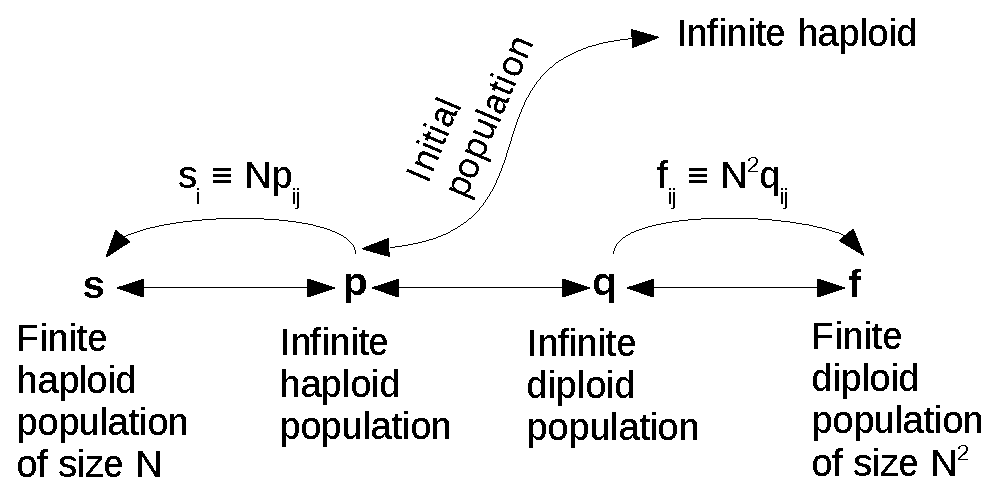
\includegraphics{figures/eps/initialpop.eps}}\hspace{4pt}
\caption{\textbf{Initial population computation} }
\label{initialpop}
\end{center}
\end{figure}

Let finite haploid population $\bm{s}^n$, finite diploid population $\bm{f}^n$, infinite haploid population $\bm{p}^n$ 
and infinite haploid population $\bm{q}^n$ be considered with initial population $\bm{s}^0$, $\bm{f}^0$,
$\bm{p}^0$, $\bm{q}^0$ respectively. To investigate oscillating behavior of infinite population evolutionary limits 
and finite population, same initial population is desired. 

For a genome length $\ell$, let $x = 2^\ell$ be number of possible strings in finite haploid population array $\bm{t}$ of 
population size $N$. Possible strings $\bm{t}_i$ are ${0, 1,.., x-1}$ where $i = 0, 1,.., N-1$. An arbitrary vector $\bm{f}$ of size $x$ 
was considered where
\[
\bm{r}_i = U01(); \tabspace {i = 0, 1,.., x-1}
\]
and U01() is random number between 0 and 1.
Let $\bm{t}$ represent finite haploid population strings array.
\[
\bm{t}_j = randp(\bm{r}) ; \tabspace {j = 0,.., N-1}
\]
where $\bm{t}_j$ is $j^{th}$ population member and $randp(\bm{r})$ returns random index $i$ in array $\bm{r}$ with probability $\bm{r}_i$.

Let $\bm{c}_i$ represent count of haploid member $i$ in population $\bm{t}$ given by
\[
\bm{c}_i = \sum \limits_{j=0}^{N-1} [\bm{t}_j = i]  \nudge; \tabspace  {i = 0,.., x-1} \text{ and  [..]  is  Iverson bracket.}
\]

Then infinite population vector $\bm{p}$ is calculated as
\[
\bm{p}_i = \frac{\bm{c}_i}{ \sum \limits_{k=0}^{x-1} \bm{c}_k }
\]
where $i = 0,.., x-1$ and $\sum \limits_{k=0}^{x-1} \bm{c}_k = N$.

This $\bm{p}$ is randomly generated initial infinite haploid population vector ($\bm{p}^0$) which corresponds to diploid infinite population vector $\bm{q}$ 
and finite population vectors $\bm{s}$ and $\bm{f}$.

Finite haploid population members $\bm{t}_j$s are generated again to match finite haploid population $\bm{s}^0$ with infinite haploid population $\bm{p}^0$.
\[
\bm{c}_i = N \cdot \bm{p}_i 
\]
\[
\sum \limits_{j=0}^{N-1} [\bm{t}_j = i] = \bm{c}_i  \nudge; \tabspace  {i = 0,.., x-1} 
\]

Initial infinite diploid population $\bm{q}_0$ is calculated corresponding to initial haploid population $\bm{p}^0$ as
\[
\bm{q}_{i,j} = \bm{p}_i \cdot \bm{p}_j  \nudge; \tabspace  {i = 0,..,x-1; \tabspace j = 0,..,x-1}.
\]

Let $\bm{v}$ represent finite diploid population member array of size $N^2$ and $\bm{d}_{i,j}$ represent count of 
diploid member $\langle i,j \rangle$ in $\bm{v}$. Then $\bm{v}$ can be filled with population member to match 
initial population vector $\bm{p}$ generating diploid members such that
\begin{eqnarray*}
\bm{d}_{i,j} & = & N \cdot \bm{p}_i \cdot N \cdot \bm{p}_j  \\
\sum \limits_{k=0}^{N^2-1} [ \bm{v}_k = \langle i,j \rangle ] & = & \bm{d}_{i,j}
\end{eqnarray*}

Finite diploid population vector $\bm{f}$ can be obtained from finite diploid population member array $\bm{v}$  using
\[
f_{i,j} = \frac{\bm{d}_{i,j}}{\sum \limits_{k=0}^{x-1} \sum \limits_{h=0}^{x-1} \bm{d}_{k,h}}
\]
where $i = 0,.., x-1$, $h = 0,.., x-1$ and $\sum \limits_{k=0}^{x-1} \sum \limits_{h=0}^{x-1} \bm{d}_{k,h} = N^2$.

This initial infinite haploid population vector $\bm{p}^0$ corresponds to initial infinite diploid population vector $\bm{q}^0$, initial finite 
haploid population vector with population size $N$ and initial finite diploid population vector $N^2$ with population size $N^2$.

\section{Oscillation}
\label{Oscillation}

Equations (\ref{lt1}) and (\ref{lt2}) were implemented with crossover distribution $\bm{\chi}$ and mutation distribution $\bm{\mu}$ satisfying 
condition (\ref{OscCond}) to investigate oscillating behavior of predicted infinite population evolutionary limits $\bm{p}^{\ast}$ and $\bm{q}^{\ast}$ 
and finite population under no selective pressure.

Infinite haploid population evolutionary limits $\bm{p}_h^{\ast}$ and $\bm{q}_h^{\ast}$ were computed using equations (\ref{lt1}) and (\ref{lt2}). 
Infinite diploid population evolutionary limits $\bm{p}_d^{\ast}$ and $\bm{q}_d^{\ast}$ as
\begin{eqnarray*}
{\bm{p}_d^{\ast}}_{\langle \gamma_0, \gamma_1 \rangle} & = & {\bm{p}_h^{\ast}}_{\gamma_0} {\bm{p}_h^{\ast}}_{\gamma_1} \\
{\bm{q}_d^{\ast}}_{\langle \gamma_0, \gamma_1 \rangle} & = & {\bm{q}_h^{\ast}}_{\gamma_0} {\bm{q}_h^{\ast}}_{\gamma_1}
\end{eqnarray*}
where $\gamma = \langle \gamma_0, \gamma_1 \rangle$ is diploid genome.

For a genome length $\ell$, same initial population (calculated as described in (\ref{InitPopOsc})) was used for infinite population and all 
sizes of finite population conisdered.
Genome lengths $\ell = \{8, \nudge10, \nudge12, \nudge14\}$ were used. Base population size of $N_0 = 64$ was considered for finite haploid case and 
different population sizes $N = \{1N_0^2, \nudge10N_0^2, \nudge20N_0^2\}$ were considered for plotting graphs. 
The distances of $\bm{p}^n$ and $\bm{s}^n$ to haploid evolutionary limits $\bm{p}_h^{\ast}$ and $\bm{q}_h^{\ast}$ were plotted and the distances of $\bm{q}^n$ and 
$\bm{f}^n$ to diploid evolutionary limits $\bm{p}_d^{\ast}$ and $\bm{q}_d^{\ast}$ were plotted. Distance data of finite population to infinite population were also plotted.


%oscillation


% l = 8
\begin{figure}[H]
\begin{center}
\subfloat{
\resizebox{8cm}{5cm}{\includegraphics{figures/eps/osc/b8/n004096_osc_fin_hap.eps}}} \hspace{-3em}% 
\subfloat{
\resizebox{8cm}{5cm}{\includegraphics{figures/eps/osc/b8/n004096_osc_fin_hap_dist.eps}}} \vspace{-1em}  \hspace{-3em}% 

\end{center}
\begin{center}
\subfloat{
\resizebox{8cm}{5cm}{\includegraphics{figures/eps/osc/b8/n040960_osc_fin_hap.eps}}} \hspace{-3em}% 
\subfloat{
\resizebox{8cm}{5cm}{\includegraphics{figures/eps/osc/b8/n040960_osc_fin_hap_dist.eps}}} \vspace{-1em}  \hspace{-3em}% 
\end{center}

\begin{center}
\subfloat{
\resizebox{8cm}{5cm}{\includegraphics{figures/eps/osc/b8/n081920_osc_fin_hap.eps}}} \hspace{-3em}% 
\subfloat{
\resizebox{8cm}{5cm}{\includegraphics{figures/eps/osc/b8/n081920_osc_fin_hap_dist.eps}}} \vspace{-1em}  \hspace{-3em}% 
\end{center}


\begin{center}
\subfloat{
\resizebox{8cm}{5cm}{\includegraphics{figures/eps/osc/b8/osc_inf_hap.eps}}} \hspace{-3em}%
\subfloat{
\resizebox{8cm}{5cm}{\includegraphics{figures/eps/osc/b8/fin_hap_dist.eps}}} \vspace{-0.5em} \hspace{-3em}%

\caption{\textbf{Infinite and finite haploid population oscillation behavior for genome length $\ell = 8$ (bits):} In left column, $d$ is
  distance of finite population of size $n$ or infinite population to limits for $g$ generations. In right column, $d$ is 
  distance of finite population to infinite population for $g$ generations and $d_{avg}$ is average of distance from $1$ to $50$ generations.}
\label{oscillation_8h}
\end{center}
\end{figure}


\begin{figure}[H]

\begin{center}
\subfloat{
\resizebox{8cm}{5cm}{\includegraphics{figures/eps/osc/b8/n004096_osc_fin_dip.eps}}} \hspace{-3em}% 
\subfloat{
\resizebox{8cm}{5cm}{\includegraphics{figures/eps/osc/b8/n004096_osc_fin_dip_dist.eps}}}  \vspace{-1em}  \hspace{-3em}% 
\end{center}
\begin{center}
\subfloat{
\resizebox{8cm}{5cm}{\includegraphics{figures/eps/osc/b8/n040960_osc_fin_dip.eps}}} \hspace{-3em}% 
\subfloat{
\resizebox{8cm}{5cm}{\includegraphics{figures/eps/osc/b8/n040960_osc_fin_dip_dist.eps}}}  \vspace{-1em}  \hspace{-3em}% 
\end{center}

\begin{center}
\subfloat{
\resizebox{8cm}{5cm}{\includegraphics{figures/eps/osc/b8/n081920_osc_fin_dip.eps}}} \hspace{-3em}% 
\subfloat{
\resizebox{8cm}{5cm}{\includegraphics{figures/eps/osc/b8/n081920_osc_fin_dip_dist.eps}}}  \vspace{-1em}  \hspace{-3em}% 
\end{center}

\begin{center}
\subfloat{
\resizebox{8cm}{5cm}{\includegraphics{figures/eps/osc/b8/osc_inf_dip.eps}}} \hspace{-3em}%
\subfloat{
\resizebox{8cm}{5cm}{\includegraphics{figures/eps/osc/b8/fin_dip_dist.eps}}} \vspace{-0.5em} \hspace{-3em}%

\caption{\textbf{Infinite and finite diploid population oscillation behavior for genome length $\ell = 8$ (bits):} In left column, $d$ is
  distance of finite population of size $n$ or infinite population to limits for $g$ generations. In right column, $d$ is 
  distance of finite population to infinite population for $g$ generations and $d_{avg}$ is average of distance from $1$ to $50$ generations..}
\label{oscillation_8d}
\end{center}
\end{figure}

% l = 10

\begin{figure}[H]

\begin{center}
\subfloat{
\resizebox{8cm}{5cm}{\includegraphics{figures/eps/osc/b10/n004096_osc_fin_hap.eps}}} \hspace{-3em}% 
\subfloat{
\resizebox{8cm}{5cm}{\includegraphics{figures/eps/osc/b10/n004096_osc_fin_hap_dist.eps}}} \vspace{-1em}  \hspace{-3em}% 
\end{center}
\begin{center}
\subfloat{
\resizebox{8cm}{5cm}{\includegraphics{figures/eps/osc/b10/n040960_osc_fin_hap.eps}}} \hspace{-3em}% 
\subfloat{
\resizebox{8cm}{5cm}{\includegraphics{figures/eps/osc/b10/n040960_osc_fin_hap_dist.eps}}} \vspace{-1em}  \hspace{-3em}% 
\end{center}

\begin{center}
\subfloat{
\resizebox{8cm}{5cm}{\includegraphics{figures/eps/osc/b10/n081920_osc_fin_hap.eps}}} \hspace{-3em}% 
\subfloat{
\resizebox{8cm}{5cm}{\includegraphics{figures/eps/osc/b10/n081920_osc_fin_hap_dist.eps}}} \vspace{-1em}  \hspace{-3em}% 
\end{center}

\begin{center}
\subfloat{
\resizebox{8cm}{5cm}{\includegraphics{figures/eps/osc/b10/osc_inf_hap.eps}}} \hspace{-3em}%
\subfloat{
\resizebox{8cm}{5cm}{\includegraphics{figures/eps/osc/b10/fin_hap_dist.eps}}} \vspace{-0.5em} \hspace{-3em}%

\caption{\textbf{Infinite and finite haploid population oscillation behavior for genome length $\ell = 10$ (bits):} In left column, $d$ is
  distance of finite population of size $n$ or infinite population to limits for $g$ generations. In right column, $d$ is 
  distance of finite population to infinite population for $g$ generations and $d_{avg}$ is average of distance from $1$ to $50$ generations..}
\label{oscillation_10h}
\end{center}
\end{figure}


\begin{figure}[H]

\begin{center}
\subfloat{
\resizebox{8cm}{5cm}{\includegraphics{figures/eps/osc/b10/n004096_osc_fin_dip.eps}}} \hspace{-3em}% 
\subfloat{
\resizebox{8cm}{5cm}{\includegraphics{figures/eps/osc/b10/n004096_osc_fin_dip_dist.eps}}}  \vspace{-1em}  \hspace{-3em}% 
\end{center}
\begin{center}
\subfloat{
\resizebox{8cm}{5cm}{\includegraphics{figures/eps/osc/b10/n040960_osc_fin_dip.eps}}} \hspace{-3em}% 
\subfloat{
\resizebox{8cm}{5cm}{\includegraphics{figures/eps/osc/b10/n040960_osc_fin_dip_dist.eps}}}  \vspace{-1em}  \hspace{-3em}% 
\end{center}

\begin{center}
\subfloat{
\resizebox{8cm}{5cm}{\includegraphics{figures/eps/osc/b10/n081920_osc_fin_dip.eps}}} \hspace{-3em}% 
\subfloat{
\resizebox{8cm}{5cm}{\includegraphics{figures/eps/osc/b10/n081920_osc_fin_dip_dist.eps}}}  \vspace{-1em}  \hspace{-3em}% 
\end{center}


\begin{center}
\subfloat{
\resizebox{8cm}{5cm}{\includegraphics{figures/eps/osc/b10/osc_inf_dip.eps}}} \hspace{-3em}%
\subfloat{
\resizebox{8cm}{5cm}{\includegraphics{figures/eps/osc/b10/fin_dip_dist.eps}}} \vspace{-0.5em} \hspace{-3em}%

\caption{\textbf{Infinite and finite population oscillation behavior for genome length $\ell = 10$ (bits):} In left column, $d$ is
  distance of finite population of size $n$ or infinite population to limits for $g$ generations. In right column, $d$ is 
  distance of finite population to infinite population for $g$ generations and $d_{avg}$ is average of distance from $1$ to $50$ generations..}
\label{oscillation_10d}
\end{center}
\end{figure}

% l = 12

\begin{figure}[H]

\begin{center}
\subfloat{
\resizebox{8cm}{5cm}{\includegraphics{figures/eps/osc/b12/n004096_osc_fin_hap.eps}}} \hspace{-3em}% 
\subfloat{
\resizebox{8cm}{5cm}{\includegraphics{figures/eps/osc/b12/n004096_osc_fin_hap_dist.eps}}} \vspace{-1em}  \hspace{-3em}% 
\end{center}
\begin{center}
\subfloat{
\resizebox{8cm}{5cm}{\includegraphics{figures/eps/osc/b12/n040960_osc_fin_hap.eps}}} \hspace{-3em}% 
\subfloat{
\resizebox{8cm}{5cm}{\includegraphics{figures/eps/osc/b12/n040960_osc_fin_hap_dist.eps}}} \vspace{-1em}  \hspace{-3em}% 
\end{center}
\begin{center}
\subfloat{
\resizebox{8cm}{5cm}{\includegraphics{figures/eps/osc/b12/n081920_osc_fin_hap.eps}}} \hspace{-3em}% 
\subfloat{
\resizebox{8cm}{5cm}{\includegraphics{figures/eps/osc/b12/n081920_osc_fin_hap_dist.eps}}} \vspace{-1em}  \hspace{-3em}% 
\end{center}

\begin{center}
\subfloat{
\resizebox{8cm}{5cm}{\includegraphics{figures/eps/osc/b12/osc_inf_hap.eps}}} \hspace{-3em}%
\subfloat{
\resizebox{8cm}{5cm}{\includegraphics{figures/eps/osc/b12/fin_hap_dist.eps}}} \vspace{-0.5em} \hspace{-3em}%

\caption{\textbf{Infinite and finite haploid population oscillation behavior for genome length $\ell = 12$ (bits):} In left column, $d$ is
  distance of finite population of size $n$ or infinite population to limits for $g$ generations. In right column, $d$ is 
  distance of finite population to infinite population for $g$ generations and $d_{avg}$ is average of distance from $1$ to $50$ generations..}
\label{oscillation_12h}
\end{center}
\end{figure}

\begin{figure}[H]

\begin{center}
\subfloat{
\resizebox{8cm}{5cm}{\includegraphics{figures/eps/osc/b12/n004096_osc_fin_dip.eps}}} \hspace{-3em}% 
\subfloat{
\resizebox{8cm}{5cm}{\includegraphics{figures/eps/osc/b12/n004096_osc_fin_dip_dist.eps}}}  \vspace{-1em}  \hspace{-3em}% 
\end{center}
\begin{center}
\subfloat{
\resizebox{8cm}{5cm}{\includegraphics{figures/eps/osc/b12/n040960_osc_fin_dip.eps}}} \hspace{-3em}% 
\subfloat{
\resizebox{8cm}{5cm}{\includegraphics{figures/eps/osc/b12/n040960_osc_fin_dip_dist.eps}}}  \vspace{-1em}  \hspace{-3em}% 
\end{center}

\begin{center}
\subfloat{
\resizebox{8cm}{5cm}{\includegraphics{figures/eps/osc/b12/n081920_osc_fin_dip.eps}}} \hspace{-3em}% 
\subfloat{
\resizebox{8cm}{5cm}{\includegraphics{figures/eps/osc/b12/n081920_osc_fin_dip_dist.eps}}}  \vspace{-1em}  \hspace{-3em}% 
\end{center}

\begin{center}
\subfloat{
\resizebox{8cm}{5cm}{\includegraphics{figures/eps/osc/b12/osc_inf_dip.eps}}} \hspace{-3em}%
\subfloat{
\resizebox{8cm}{5cm}{\includegraphics{figures/eps/osc/b10/fin_hap_dist.eps}}} \vspace{-0.5em} \hspace{-3em}%

\caption{\textbf{Infinite and finite diploid population oscillation behavior for genome length $\ell = 12$ (bits):} In left column, $d$ is
  distance of finite population of size $n$ or infinite population to limits for $g$ generations. In right column, $d$ is 
  distance of finite population to infinite population for $g$ generations and $d_{avg}$ is average of distance from $1$ to $50$ generations..}
\label{oscillation_12d}
\end{center}
\end{figure}


% l= 14


\begin{figure}[H]

\begin{center}
\subfloat{
\resizebox{8cm}{5cm}{\includegraphics{figures/eps/osc/b14/n004096_osc_fin_hap.eps}}} \hspace{-3em}% 
\subfloat{
\resizebox{8cm}{5cm}{\includegraphics{figures/eps/osc/b14/n004096_osc_fin_hap_dist.eps}}} \vspace{-1em}  \hspace{-3em}% 
\end{center}
\begin{center}
\subfloat{
\resizebox{8cm}{5cm}{\includegraphics{figures/eps/osc/b14/n040960_osc_fin_hap.eps}}} \hspace{-3em}% 
\subfloat{
\resizebox{8cm}{5cm}{\includegraphics{figures/eps/osc/b14/n040960_osc_fin_hap_dist.eps}}} \vspace{-1em}  \hspace{-3em}% 
\end{center}

\begin{center}
\subfloat{
\resizebox{8cm}{5cm}{\includegraphics{figures/eps/osc/b14/n081920_osc_fin_hap.eps}}} \hspace{-3em}% 
\subfloat{
\resizebox{8cm}{5cm}{\includegraphics{figures/eps/osc/b14/n081920_osc_fin_hap_dist.eps}}} \vspace{-1em}  \hspace{-3em}% 
\end{center}

\begin{center}
\subfloat{
\resizebox{8cm}{5cm}{\includegraphics{figures/eps/osc/b14/osc_inf_hap.eps}}} \hspace{-3em}%
\subfloat{
\resizebox{8cm}{5cm}{\includegraphics{figures/eps/osc/b14/fin_hap_dist.eps}}} \vspace{-0.5em} \hspace{-3em}%

\caption{\textbf{Infinite and finite haploid population oscillation behavior for genome length $\ell = 14$ (bits):} In left column, $d$ is
  distance of finite population of size $n$ or infinite population to limits for $g$ generations. In right column, $d$ is 
  distance of finite population to infinite population for $g$ generations and $d_{avg}$ is average of distance from $1$ to $50$ generations..}
\label{oscillation_14h}
\end{center}
\end{figure}

\begin{figure}[H]

\begin{center}
\subfloat{
\resizebox{8cm}{5cm}{\includegraphics{figures/eps/osc/b14/n004096_osc_fin_dip.eps}}} \hspace{-3em}% 
\subfloat{
\resizebox{8cm}{5cm}{\includegraphics{figures/eps/osc/b14/n004096_osc_fin_dip_dist.eps}}}  \vspace{-1em}  \hspace{-3em}% 
\end{center}
\begin{center}
\subfloat{
\resizebox{8cm}{5cm}{\includegraphics{figures/eps/osc/b14/n040960_osc_fin_dip.eps}}} \hspace{-3em}% 
\subfloat{
\resizebox{8cm}{5cm}{\includegraphics{figures/eps/osc/b14/n040960_osc_fin_dip_dist.eps}}}  \vspace{-1em}  \hspace{-3em}% 
\end{center}

\begin{center}
\subfloat{
\resizebox{8cm}{5cm}{\includegraphics{figures/eps/osc/b14/n081920_osc_fin_dip.eps}}} \hspace{-3em}% 
\subfloat{
\resizebox{8cm}{5cm}{\includegraphics{figures/eps/osc/b14/n081920_osc_fin_dip_dist.eps}}}  \vspace{-1em}  \hspace{-3em}% 
\end{center}

\begin{center}
\subfloat{
\resizebox{8cm}{5cm}{\includegraphics{figures/eps/osc/b14/osc_inf_dip.eps}}} \hspace{-3em}%
\subfloat{
\resizebox{8cm}{5cm}{\includegraphics{figures/eps/osc/b14/fin_dip_dist.eps}}} \vspace{-0.5em} \hspace{-3em}%

\caption{\textbf{Infinite and finite diploid population oscillation behavior for genome length $\ell = 14$ (bits):} In left column, $d$ is
  distance of finite population of size $n$ or infinite population to limits for $g$ generations. In right column, $d$ is 
  distance of finite population to infinite population for $g$ generations and $d_{avg}$ is average of distance from $1$ to $50$ generations..}
\label{oscillation_14d}
\end{center}
\end{figure}
%oscillation


\textbf{ Figures} \ref{oscillation_8h}, \ref{oscillation_8d}, \ref{oscillation_10h}, \ref{oscillation_10d}, \ref{oscillation_12h}, \ref{oscillation_12d}, 
\ref{oscillation_14h} and \ref{oscillation_14d} arranged by genome length $\ell$ 
and sub-figures within each figures arranged by population size ($N$) for finite population for haploid and diploid population 
depticts oscillating behavior of both infinite and finite population when necessary and sufficient condition \ref{OscCond} is met. 
Oscillation in finite population in both haploid and diploid case simulation became sharper with increased population size as expected. 
As size of finite population increased, oscillation behavior depicted by finite population grew analogous to oscillation behavior 
depicted by infinite population. 

Graphs of difference in distance ($d$) and  average distance ($d_{avg}$) were plotted for both haploid and diploid cas on right side of
oscillation graphs in above figures where $d$ is distance of finite population to infinite population and $d_{avg}$ is average of distance 
from $1^{st}$ to $50^{th}$ generation. For a given genome length $\ell$ and haploid or diploid case, single graph for distances of 
different finite population sizes ($N = 1N_0^2, \nudge10N_0^2, \nudge20N_0^2$) were plotted. 
The resulting graphs showed distance decreased as population size increased which is expected and in congruence with results from section \ref{convergence}. 
Graphs show curve of distance of finite population to infinite population smoothens as population size increased. The graphs of $d-d_{avg}$ 
shows decrease in amplitude of ripples as population size increases.

Numerator $\sqrt{(1 - \|\mathcal{G}(\bm{p})\|^2)}$ in equation \ref{convergenceRHS} is calculated using initial population and is $\approx 1$. 
So from \ref{convergenceRHS}, the expected single step distance between finite and infinite population, $d$, can be approximated as
\[
d \approx 1/\sqrt{N}
\]
where $N$ is size of finite population.
Then mathematical expection of single step distance for finite population size $N = \{4096, \nudge 40960, \nudge 81920\}$ considered for plotting is shown in following table.
\begin{table}[ht]
\caption{\textbf{Expected single step distance $d$ for population size $N$}}
\centering
\begin{tabular}{c c c c}
\hline
$N$ & 4096 & 40960 & 81920 \\
$d$ & 0.015625 & 0.004941 & 0.003494 \\
\hline
\end{tabular}
\label{tableExpectedDistance}
\end{table}

Data obtained from distances of finite population of size $N = \{4096, \nudge 40960, \nudge 81920\}$ to infinite population obtained from simulation 
for oscillation for both haploid and dioploid case with genome length $\ell = \{8, \nudge 10, \nudge 12, \nudge 14\}$ are tabulated below.
%\newpage
\begin{table}[ht]
\caption{\textbf{Experimental distance measured for oscillation:} $N$ is finite population size, $\ell$ is genome length and $\{d^\prime, d^{\prime\prime}, d^{\prime\prime\prime}\}$ are distances to infinite population from finite population of sizes $\{4096, \nudge 40960, \nudge 81920\}$ }
\centering
\begin{tabularx}{0.75\textwidth}{ c *{4}{X}}
\toprule
case & $\ell$ & $d^\prime$ & $d^{\prime\prime}$ & $d^{\prime\prime\prime}$\\
\midrule
\multirow{4}{*}{haploid} 	& 8 & 0.015785 & 0.005123 & 0.003559 \\
 				& 10 & 0.015663 & 0.005007 & 0.003511 \\ 
 			 	& 12 & 0.015638 & 0.004933 & 0.003497 \\
 	 			& 14 & 0.015626 & 0.004948 & 0.003503 \\ 
\midrule
\multirow{4}{*}{diploid} 	& 8 & 0.015623 & 0.004942 & 0.003498 \\
				& 10 & 0.015624 & 0.004941 & 0.003494 \\
			 	& 12 & 0.015625 & 0.004941 & 0.003494 \\
	 			& 14 & 0.015625 & 0.004941 & 0.003494 \\
\bottomrule

\end{tabularx}
\label{tableDistanceOsc}
\end{table}


From table \ref{tableDistanceOsc}, averaged distances obtained for finite population size $N = \{4096,  40960,  81920\}$ are $\{0.015651, 0.004972, 0.003506\} $ respectively.
The results from table \ref{tableDistanceOsc} shows the distance between finite population and infinite population, although measured over number of generations, follows closely 
the expected single step distance between finite and infinite population given by  table \ref{tableExpectedDistance} and the distance decreased as $1/\sqrt{N}$.

\section{Violation}

The results showed when $\bm{\chi}$ and $\bm{\mu}$ distributions satisfies (\ref{OscCond}), oscillation occurs in both infinite and finite population. 
Error $\bm{\epsilon}$ was introduced to $\bm{\mu}$ distribution and $\bm{\chi}$ distribution such that (\ref{OscCond}) did not satisfy anymore and 
$x_g \neq −1$ for all $g$ ($x_g$ and $g$ defined in \ref{Limits}) so that $\bm{p}^\ast = \bm{q}^\ast$.

In this section, operations ($+$ and $\cdot$) acting on elements of $\mathcal{R}$ are component-wise addition and multiplication modulo 2. 

$\bm{\mu}$ distribution was treated with $\bm{\epsilon}$ such that
\[
\bm{\mu}_i = (1-\bm{\epsilon}) \bm{\mu}_i \nudge; \tabspace i = \{0, 1, 2,.., 2^{\ell}-1\}.
\]
So that sum of $\bm{\mu}$ distribution becomes, 
\[
1-\bm{\epsilon} = \sum \limits_{i=0}^{2^{\ell}-1} \bm{\mu}_i
\]
Then set
\[
\bm{\mu}_0 = \bm{\epsilon}
\]

$\bm{\chi}$ distribution was treated with $\bm{\epsilon}$ such that
\[
\bm{\chi}_i = (1-\bm{\epsilon}) \bm{\chi} ; \tabspace i = \{1, 2,.., 2^{\ell}-1\} 
\]
So that 
\[
\bm{\chi}_i + \bm{\chi}_{i+g} = 1-\bm{\epsilon} ; \tabspace g \text{ is defined in  section } \ref{Limits}
\]

Then $j$ is chosen where $\bm{\chi}_j = 0$ and set $\bm{\chi}_j = \bm{\epsilon}$. \newline

Simulations were run again with violations in (\ref{OscCond}) implemented. Genome lengths  $\ell = \{8, \nudge 10, \nudge 12, \nudge 14\}$ were considered. 
Different finite hapliod population sizes $N = \{1N_0^2, \nudge 10N_0^2, \nudge 20N_0^2\}$ were considered. 
\newline
Let ${\bm{p}1}^{\ast}$ and ${\bm{q}1}^{\ast}$ be evolutionary limits with violation, 
then ${\bm{p}1}^{\ast} = {\bm{q}1}^{\ast} = {\bm{z}}^\ast$; $\bm{z}^\ast$ is limit when there is violation.
The distances of ${p}^n$ and $\bm{s}^n$ to $\bm{z}^\ast$ were plotted and the distances of 
$\bm{q}^n$ and $\bm{f}^n$ to $\bm{z}^\ast$ were plotted from $1^{st}$ to $50^{th}$ generations. The distances of population to evolutionary limits that would be 
without violation in $\bm{\mu}$ and $\bm{\chi}$ were also plotted from $1^{st}$ to $50^{th}$ generations.


% figures for mu violation
\input{chapters/violation-mu.tex}

% figures for chi violation

% l = 8

\begin{figure}[H]
\begin{center}
\subfloat{
\resizebox{8cm}{5cm}{\includegraphics{figures/eps/vio/chi/b8/e0.01/n004096_fin_hap.eps}}} \hspace{-3em}%
\subfloat{
\resizebox{8cm}{5cm}{\includegraphics{figures/eps/vio/chi/b8/e0.01/n004096_fin_hap_wovio.eps}}}\vspace{-1em} \hspace{-3em}%
\end{center}
\begin{center}
\subfloat{
\resizebox{8cm}{5cm}{\includegraphics{figures/eps/vio/chi/b8/e0.01/n102400_fin_hap.eps}}} \hspace{-3em}%
\subfloat{
\resizebox{8cm}{5cm}{\includegraphics{figures/eps/vio/chi/b8/e0.01/n102400_fin_hap_wovio.eps}}}\vspace{-1em} \hspace{-3em}%
\end{center}

\begin{center}
\subfloat{
\resizebox{8cm}{5cm}{\includegraphics{figures/eps/vio/chi/b8/e0.01/n1048576_fin_hap.eps}}} \hspace{-3em}%
\subfloat{
\resizebox{8cm}{5cm}{\includegraphics{figures/eps/vio/chi/b8/e0.01/n1048576_fin_hap_wovio.eps}}}\vspace{-1em} \hspace{-3em}%
\end{center}

\begin{center}
\subfloat{
\resizebox{8cm}{5cm}{\includegraphics{figures/eps/vio/chi/b8/e0.01/inf_hap.eps}}}\hspace{-3em}%
\subfloat{
\resizebox{8cm}{5cm}{\includegraphics{figures/eps/vio/chi/b8/e0.01/inf_hap_wovio.eps}}}\vspace{-0.5em} \hspace{-3em}%


\caption{\textbf{Infinite and finite haploid population oscillation behavior in case of violation in $\bm{\chi}$ for genome length $\ell = 8$ and $\epsilon = 0.01$:} 
  $d$ is distance between infinite or finite population of size $N$ and infinite
  population limits for $g$ generations. $d$ in left column is distance to limits with violation
  and in right column is distance to limits without violation.}
\label{oscillation_8h_vio_chi_0.01}
\end{center}
\end{figure}

\begin{figure}[H]
\begin{center}
\subfloat{
\resizebox{8cm}{5cm}{\includegraphics{figures/eps/vio/chi/b8/e0.01/n004096_fin_dip.eps}}}\hspace{-3em}%
\subfloat{
\resizebox{8cm}{5cm}{\includegraphics{figures/eps/vio/chi/b8/e0.01/n004096_fin_dip_wovio.eps}}}\vspace{-1em}  \hspace{-3em}%
\end{center}
\begin{center}
\subfloat{
\resizebox{8cm}{5cm}{\includegraphics{figures/eps/vio/chi/b8/e0.01/n102400_fin_dip.eps}}}\hspace{-3em}%
\subfloat{
\resizebox{8cm}{5cm}{\includegraphics{figures/eps/vio/chi/b8/e0.01/n102400_fin_dip_wovio.eps}}}\vspace{-1em}  \hspace{-3em}%
\end{center}


\begin{center}
\subfloat{
\resizebox{8cm}{5cm}{\includegraphics{figures/eps/vio/chi/b8/e0.01/n1048576_fin_dip.eps}}}\hspace{-3em}%
\subfloat{
\resizebox{8cm}{5cm}{\includegraphics{figures/eps/vio/chi/b8/e0.01/n1048576_fin_dip_wovio.eps}}}\vspace{-1em}  \hspace{-3em}%
\end{center}

\begin{center}
\subfloat{
\resizebox{8cm}{5cm}{\includegraphics{figures/eps/vio/chi/b8/e0.01/inf_dip.eps}}}\hspace{-3em}%
\subfloat{
\resizebox{8cm}{5cm}{\includegraphics{figures/eps/vio/chi/b8/e0.01/inf_dip_wovio.eps}}}\vspace{-0.5em}  \hspace{-3em}%


\caption{\textbf{Infinite and finite diploid population oscillation behavior in case of violation in $\bm{\chi}$ for genome length $\ell = 8$ and $\epsilon = 0.01$:} 
  $d$ is distance between infinite or finite population of size $N$ and infinite
  population limits for $g$ generations. $d$ in left column is distance to limits with violation
  and in right column is distance to limits without violation.}
\label{oscillation_8d_vio_chi_0.01}
\end{center}
\end{figure}



\begin{figure}[H]
\begin{center}
\subfloat{
\resizebox{8cm}{5cm}{\includegraphics{figures/eps/vio/chi/b8/e0.1/n004096_fin_hap.eps}}}  \hspace{-3em}%
\subfloat{
\resizebox{8cm}{5cm}{\includegraphics{figures/eps/vio/chi/b8/e0.1/n004096_fin_hap_wovio.eps}}}\vspace{-1em}  \hspace{-3em}%
\end{center}
\begin{center}
\subfloat{
\resizebox{8cm}{5cm}{\includegraphics{figures/eps/vio/chi/b8/e0.1/n102400_fin_hap.eps}}}  \hspace{-3em}%
\subfloat{
\resizebox{8cm}{5cm}{\includegraphics{figures/eps/vio/chi/b8/e0.1/n102400_fin_hap_wovio.eps}}}\vspace{-1em}  \hspace{-3em}%
\end{center}

\begin{center}
\subfloat{
\resizebox{8cm}{5cm}{\includegraphics{figures/eps/vio/chi/b8/e0.1/n1048576_fin_hap.eps}}}  \hspace{-3em}%
\subfloat{
\resizebox{8cm}{5cm}{\includegraphics{figures/eps/vio/chi/b8/e0.1/n1048576_fin_hap_wovio.eps}}}\vspace{-1em}  \hspace{-3em}%
\end{center}

\begin{center}
\subfloat{
\resizebox{8cm}{5cm}{\includegraphics{figures/eps/vio/chi/b8/e0.1/inf_hap.eps}}} \hspace{-3em}%
\subfloat{
\resizebox{8cm}{5cm}{\includegraphics{figures/eps/vio/chi/b8/e0.1/inf_hap_wovio.eps}}}\vspace{-0.5em}  \hspace{-3em}%


\caption{\textbf{Infinite and finite haploid population oscillation behavior in case of violation in $\bm{\chi}$ for genome length $\ell = 8$ and $\epsilon = 0.1$:} 
  $d$ is distance between infinite or finite population of size $N$ and infinite
  population limits for $g$ generations. $d$ in left column is distance to limits with violation
  and in right column is distance to limits without violation.}
\label{oscillation_8h_vio_chi_0.1}
\end{center}
\end{figure}

\begin{figure}[H]
\begin{center}
\subfloat{
\resizebox{8cm}{5cm}{\includegraphics{figures/eps/vio/chi/b8/e0.1/n004096_fin_dip.eps}}}\hspace{-3em}%
\subfloat{
\resizebox{8cm}{5cm}{\includegraphics{figures/eps/vio/chi/b8/e0.1/n004096_fin_dip_wovio.eps}}}\vspace{-1em}  \hspace{-3em}%
\end{center}
\begin{center}
\subfloat{
\resizebox{8cm}{5cm}{\includegraphics{figures/eps/vio/chi/b8/e0.1/n102400_fin_dip.eps}}}\hspace{-3em}%
\subfloat{
\resizebox{8cm}{5cm}{\includegraphics{figures/eps/vio/chi/b8/e0.1/n102400_fin_dip_wovio.eps}}}\vspace{-1em}  \hspace{-3em}%
\end{center}

\begin{center}
\subfloat{
\resizebox{8cm}{5cm}{\includegraphics{figures/eps/vio/chi/b8/e0.1/n1048576_fin_dip.eps}}}\hspace{-3em}%
\subfloat{
\resizebox{8cm}{5cm}{\includegraphics{figures/eps/vio/chi/b8/e0.1/n1048576_fin_dip_wovio.eps}}}\vspace{-1em}  \hspace{-3em}%
\end{center}

\begin{center}
\subfloat{
\resizebox{8cm}{5cm}{\includegraphics{figures/eps/vio/chi/b8/e0.1/inf_dip.eps}}}\hspace{-3em}%
\subfloat{
\resizebox{8cm}{5cm}{\includegraphics{figures/eps/vio/chi/b8/e0.1/inf_dip_wovio.eps}}}\vspace{-0.5em}  \hspace{-3em}%


\caption{\textbf{Infinite and finite diploid population oscillation behavior in case of violation in $\bm{\chi}$ for genome length $\ell = 8$ and $\epsilon = 0.1$:} 
  $d$ is distance between infinite or finite population of size $N$ and infinite
  population limits for $g$ generations. $d$ in left column is distance to limits with violation
  and in right column is distance to limits without violation.}
\label{oscillation_8d_vio_chi_0.1}
\end{center}
\end{figure}


\begin{figure}[H]

\begin{center}
\subfloat{
\resizebox{8cm}{5cm}{\includegraphics{figures/eps/vio/chi/b8/e0.5/n004096_fin_hap.eps}}}  \hspace{-3em}%
\subfloat{
\resizebox{8cm}{5cm}{\includegraphics{figures/eps/vio/chi/b8/e0.5/n004096_fin_hap_wovio.eps}}}\vspace{-1em}  \hspace{-3em}%
\end{center}
\begin{center}
\subfloat{
\resizebox{8cm}{5cm}{\includegraphics{figures/eps/vio/chi/b8/e0.5/n102400_fin_hap.eps}}}  \hspace{-3em}%
\subfloat{
\resizebox{8cm}{5cm}{\includegraphics{figures/eps/vio/chi/b8/e0.5/n102400_fin_hap_wovio.eps}}}\vspace{-1em}  \hspace{-3em}%
\end{center}

\begin{center}
\subfloat{
\resizebox{8cm}{5cm}{\includegraphics{figures/eps/vio/chi/b8/e0.5/n1048576_fin_hap.eps}}}  \hspace{-3em}%
\subfloat{
\resizebox{8cm}{5cm}{\includegraphics{figures/eps/vio/chi/b8/e0.5/n1048576_fin_hap_wovio.eps}}}\vspace{-1em}  \hspace{-3em}%
\end{center}

\begin{center}
\subfloat{
\resizebox{8cm}{5cm}{\includegraphics{figures/eps/vio/chi/b8/e0.5/inf_hap.eps}}} \hspace{-3em}%
\subfloat{
\resizebox{8cm}{5cm}{\includegraphics{figures/eps/vio/chi/b8/e0.5/inf_hap_wovio.eps}}}\vspace{-0.5em}  \hspace{-3em}%


\caption{\textbf{Infinite and finite haploid population oscillation behavior in case of violation in $\bm{\chi}$ for 
  genome length $\ell = 8$ and $\epsilon = 0.5$:} $d$ is distance between infinite or finite population of size $N$ and infinite
  population limits for $g$ generations. $d$ in left column is distance to limits with violation
  and in right column is distance to limits without violation.}
\label{oscillation_8h_vio_chi_0.5}
\end{center}
\end{figure}

\begin{figure}[H]
\begin{center}
\subfloat{
\resizebox{8cm}{5cm}{\includegraphics{figures/eps/vio/chi/b8/e0.5/n004096_fin_dip.eps}}}\hspace{-3em}%
\subfloat{
\resizebox{8cm}{5cm}{\includegraphics{figures/eps/vio/chi/b8/e0.5/n004096_fin_dip_wovio.eps}}}\vspace{-1em}  \hspace{-3em}%
\end{center}
\begin{center}
\subfloat{
\resizebox{8cm}{5cm}{\includegraphics{figures/eps/vio/chi/b8/e0.5/n102400_fin_dip.eps}}}\hspace{-3em}%
\subfloat{
\resizebox{8cm}{5cm}{\includegraphics{figures/eps/vio/chi/b8/e0.5/n102400_fin_dip_wovio.eps}}}\vspace{-1em}  \hspace{-3em}%
\end{center}

\begin{center}
\subfloat{
\resizebox{8cm}{5cm}{\includegraphics{figures/eps/vio/chi/b8/e0.5/n1048576_fin_dip.eps}}}\hspace{-3em}%
\subfloat{
\resizebox{8cm}{5cm}{\includegraphics{figures/eps/vio/chi/b8/e0.5/n1048576_fin_dip_wovio.eps}}}\vspace{-1em}  \hspace{-3em}%
\end{center}

\begin{center}
\subfloat{
\resizebox{8cm}{5cm}{\includegraphics{figures/eps/vio/chi/b8/e0.5/inf_dip.eps}}}\hspace{-3em}%
\subfloat{
\resizebox{8cm}{5cm}{\includegraphics{figures/eps/vio/chi/b8/e0.5/inf_dip_wovio.eps}}}\vspace{-0.5em}  \hspace{-3em}%


\caption{\textbf{Infinite and finite diploid population oscillation behavior in case of violation in $\bm{\chi}$ for genome length $\ell = 8$ and $\epsilon = 0.5$:} 
  $d$ is distance between infinite or finite population of size $N$ and infinite
  population limits for $g$ generations. $d$ in left column is distance to limits with violation
  and in right column is distance to limits without violation.}
\label{oscillation_8d_vio_chi_0.5}
\end{center}
\end{figure}


% l = 10

\begin{figure}[H]
\begin{center}
\subfloat{
\resizebox{8cm}{5cm}{\includegraphics{figures/eps/vio/chi/b10/e0.01/n004096_fin_hap.eps}}} \hspace{-3em}%
\subfloat{
\resizebox{8cm}{5cm}{\includegraphics{figures/eps/vio/chi/b10/e0.01/n004096_fin_hap_wovio.eps}}}\vspace{-1em} \hspace{-3em}%
\end{center}
\begin{center}
\subfloat{
\resizebox{8cm}{5cm}{\includegraphics{figures/eps/vio/chi/b10/e0.01/n102400_fin_hap.eps}}} \hspace{-3em}%
\subfloat{
\resizebox{8cm}{5cm}{\includegraphics{figures/eps/vio/chi/b10/e0.01/n102400_fin_hap_wovio.eps}}}\vspace{-1em} \hspace{-3em}%
\end{center}

\begin{center}
\subfloat{
\resizebox{8cm}{5cm}{\includegraphics{figures/eps/vio/chi/b10/e0.01/n1048576_fin_hap.eps}}} \hspace{-3em}%
\subfloat{
\resizebox{8cm}{5cm}{\includegraphics{figures/eps/vio/chi/b10/e0.01/n1048576_fin_hap_wovio.eps}}}\vspace{-1em} \hspace{-3em}%
\end{center}

\begin{center}
\subfloat{
\resizebox{8cm}{5cm}{\includegraphics{figures/eps/vio/chi/b10/e0.01/inf_hap.eps}}}\hspace{-3em}%
\subfloat{
\resizebox{8cm}{5cm}{\includegraphics{figures/eps/vio/chi/b10/e0.01/inf_hap_wovio.eps}}}\vspace{-0.5em} \hspace{-3em}%


\caption{\textbf{Infinite and finite haploid population oscillation behavior in case of violation in $\bm{\chi}$ for genome length $\ell = 10$ and $\epsilon = 0.01$:} 
  $d$ is distance between infinite or finite population of size $N$ and infinite
  population limits for $g$ generations. $d$ in left column is distance to limits with violation
  and in right column is distance to limits without violation.}
\label{oscillation_10h_vio_chi_0.01}
\end{center}
\end{figure}

\begin{figure}[H]
\begin{center}
\subfloat{
\resizebox{8cm}{5cm}{\includegraphics{figures/eps/vio/chi/b10/e0.01/n004096_fin_dip.eps}}}\hspace{-3em}%
\subfloat{
\resizebox{8cm}{5cm}{\includegraphics{figures/eps/vio/chi/b10/e0.01/n004096_fin_dip_wovio.eps}}}\vspace{-1em}  \hspace{-3em}%
\end{center}
\begin{center}
\subfloat{
\resizebox{8cm}{5cm}{\includegraphics{figures/eps/vio/chi/b10/e0.01/n102400_fin_dip.eps}}}\hspace{-3em}%
\subfloat{
\resizebox{8cm}{5cm}{\includegraphics{figures/eps/vio/chi/b10/e0.01/n102400_fin_dip_wovio.eps}}}\vspace{-1em}  \hspace{-3em}%
\end{center}


\begin{center}
\subfloat{
\resizebox{8cm}{5cm}{\includegraphics{figures/eps/vio/chi/b10/e0.01/n1048576_fin_dip.eps}}}\hspace{-3em}%
\subfloat{
\resizebox{8cm}{5cm}{\includegraphics{figures/eps/vio/chi/b10/e0.01/n1048576_fin_dip_wovio.eps}}}\vspace{-1em}  \hspace{-3em}%
\end{center}

\begin{center}
\subfloat{
\resizebox{8cm}{5cm}{\includegraphics{figures/eps/vio/chi/b10/e0.01/inf_dip.eps}}}\hspace{-3em}%
\subfloat{
\resizebox{8cm}{5cm}{\includegraphics{figures/eps/vio/chi/b10/e0.01/inf_dip_wovio.eps}}}\vspace{-0.5em}  \hspace{-3em}%


\caption{\textbf{Infinite and finite diploid population oscillation behavior in case of violation in $\bm{\chi}$ for genome length $\ell = 10$ and $\epsilon = 0.01$:} 
  $d$ is distance between infinite or finite population of size $N$ and infinite
  population limits for $g$ generations. $d$ in left column is distance to limits with violation
  and in right column is distance to limits without violation.}
\label{oscillation_10d_vio_chi_0.01}
\end{center}
\end{figure}



\begin{figure}[H]
\begin{center}
\subfloat{
\resizebox{8cm}{5cm}{\includegraphics{figures/eps/vio/chi/b10/e0.1/n004096_fin_hap.eps}}}  \hspace{-3em}%
\subfloat{
\resizebox{8cm}{5cm}{\includegraphics{figures/eps/vio/chi/b10/e0.1/n004096_fin_hap_wovio.eps}}}\vspace{-1em}  \hspace{-3em}%
\end{center}
\begin{center}
\subfloat{
\resizebox{8cm}{5cm}{\includegraphics{figures/eps/vio/chi/b10/e0.1/n102400_fin_hap.eps}}}  \hspace{-3em}%
\subfloat{
\resizebox{8cm}{5cm}{\includegraphics{figures/eps/vio/chi/b10/e0.1/n102400_fin_hap_wovio.eps}}}\vspace{-1em}  \hspace{-3em}%
\end{center}

\begin{center}
\subfloat{
\resizebox{8cm}{5cm}{\includegraphics{figures/eps/vio/chi/b10/e0.1/n1048576_fin_hap.eps}}}  \hspace{-3em}%
\subfloat{
\resizebox{8cm}{5cm}{\includegraphics{figures/eps/vio/chi/b10/e0.1/n1048576_fin_hap_wovio.eps}}}\vspace{-1em}  \hspace{-3em}%
\end{center}

\begin{center}
\subfloat{
\resizebox{8cm}{5cm}{\includegraphics{figures/eps/vio/chi/b10/e0.1/inf_hap.eps}}} \hspace{-3em}%
\subfloat{
\resizebox{8cm}{5cm}{\includegraphics{figures/eps/vio/chi/b10/e0.1/inf_hap_wovio.eps}}}\vspace{-0.5em}  \hspace{-3em}%


\caption{\textbf{Infinite and finite haploid population oscillation behavior in case of violation in $\bm{\chi}$ for genome length $\ell = 10$ and $\epsilon = 0.1$:} 
  $d$ is distance between infinite or finite population of size $N$ and infinite
  population limits for $g$ generations. $d$ in left column is distance to limits with violation
  and in right column is distance to limits without violation.}
\label{oscillation_10h_vio_chi_0.1}
\end{center}
\end{figure}

\begin{figure}[H]
\begin{center}
\subfloat{
\resizebox{8cm}{5cm}{\includegraphics{figures/eps/vio/chi/b10/e0.1/n004096_fin_dip.eps}}}\hspace{-3em}%
\subfloat{
\resizebox{8cm}{5cm}{\includegraphics{figures/eps/vio/chi/b10/e0.1/n004096_fin_dip_wovio.eps}}}\vspace{-1em}  \hspace{-3em}%
\end{center}
\begin{center}
\subfloat{
\resizebox{8cm}{5cm}{\includegraphics{figures/eps/vio/chi/b10/e0.1/n102400_fin_dip.eps}}}\hspace{-3em}%
\subfloat{
\resizebox{8cm}{5cm}{\includegraphics{figures/eps/vio/chi/b10/e0.1/n102400_fin_dip_wovio.eps}}}\vspace{-1em}  \hspace{-3em}%
\end{center}

\begin{center}
\subfloat{
\resizebox{8cm}{5cm}{\includegraphics{figures/eps/vio/chi/b10/e0.1/n1048576_fin_dip.eps}}}\hspace{-3em}%
\subfloat{
\resizebox{8cm}{5cm}{\includegraphics{figures/eps/vio/chi/b10/e0.1/n1048576_fin_dip_wovio.eps}}}\vspace{-1em}  \hspace{-3em}%
\end{center}

\begin{center}
\subfloat{
\resizebox{8cm}{5cm}{\includegraphics{figures/eps/vio/chi/b10/e0.1/inf_dip.eps}}}\hspace{-3em}%
\subfloat{
\resizebox{8cm}{5cm}{\includegraphics{figures/eps/vio/chi/b10/e0.1/inf_dip_wovio.eps}}}\vspace{-0.5em}  \hspace{-3em}%


\caption{\textbf{Infinite and finite diploid population oscillation behavior in case of violation in $\bm{\chi}$ for genome length $\ell = 10$ and $\epsilon = 0.1$:} 
  $d$ is distance between infinite or finite population of size $N$ and infinite
  population limits for $g$ generations. $d$ in left column is distance to limits with violation
  and in right column is distance to limits without violation.}
\label{oscillation_10d_vio_chi_0.1}
\end{center}
\end{figure}


\begin{figure}[H]

\begin{center}
\subfloat{
\resizebox{8cm}{5cm}{\includegraphics{figures/eps/vio/chi/b10/e0.5/n004096_fin_hap.eps}}}  \hspace{-3em}%
\subfloat{
\resizebox{8cm}{5cm}{\includegraphics{figures/eps/vio/chi/b10/e0.5/n004096_fin_hap_wovio.eps}}}\vspace{-1em}  \hspace{-3em}%
\end{center}
\begin{center}
\subfloat{
\resizebox{8cm}{5cm}{\includegraphics{figures/eps/vio/chi/b10/e0.5/n102400_fin_hap.eps}}}  \hspace{-3em}%
\subfloat{
\resizebox{8cm}{5cm}{\includegraphics{figures/eps/vio/chi/b10/e0.5/n102400_fin_hap_wovio.eps}}}\vspace{-1em}  \hspace{-3em}%
\end{center}

\begin{center}
\subfloat{
\resizebox{8cm}{5cm}{\includegraphics{figures/eps/vio/chi/b10/e0.5/n1048576_fin_hap.eps}}}  \hspace{-3em}%
\subfloat{
\resizebox{8cm}{5cm}{\includegraphics{figures/eps/vio/chi/b10/e0.5/n1048576_fin_hap_wovio.eps}}}\vspace{-1em}  \hspace{-3em}%
\end{center}

\begin{center}
\subfloat{
\resizebox{8cm}{5cm}{\includegraphics{figures/eps/vio/chi/b10/e0.5/inf_hap.eps}}} \hspace{-3em}%
\subfloat{
\resizebox{8cm}{5cm}{\includegraphics{figures/eps/vio/chi/b10/e0.5/inf_hap_wovio.eps}}}\vspace{-0.5em}  \hspace{-3em}%


\caption{\textbf{Infinite and finite haploid population oscillation behavior in case of violation in $\bm{\chi}$ for 
  genome length $\ell = 10$ and $\epsilon = 0.5$:} $d$ is distance between infinite or finite population of size $N$ and infinite
  population limits for $g$ generations. $d$ in left column is distance to limits with violation
  and in right column is distance to limits without violation.}
\label{oscillation_10h_vio_chi_0.5}
\end{center}
\end{figure}

\begin{figure}[H]
\begin{center}
\subfloat{
\resizebox{8cm}{5cm}{\includegraphics{figures/eps/vio/chi/b10/e0.5/n004096_fin_dip.eps}}}\hspace{-3em}%
\subfloat{
\resizebox{8cm}{5cm}{\includegraphics{figures/eps/vio/chi/b10/e0.5/n004096_fin_dip_wovio.eps}}}\vspace{-1em}  \hspace{-3em}%
\end{center}
\begin{center}
\subfloat{
\resizebox{8cm}{5cm}{\includegraphics{figures/eps/vio/chi/b10/e0.5/n102400_fin_dip.eps}}}\hspace{-3em}%
\subfloat{
\resizebox{8cm}{5cm}{\includegraphics{figures/eps/vio/chi/b10/e0.5/n102400_fin_dip_wovio.eps}}}\vspace{-1em}  \hspace{-3em}%
\end{center}

\begin{center}
\subfloat{
\resizebox{8cm}{5cm}{\includegraphics{figures/eps/vio/chi/b10/e0.5/n1048576_fin_dip.eps}}}\hspace{-3em}%
\subfloat{
\resizebox{8cm}{5cm}{\includegraphics{figures/eps/vio/chi/b10/e0.5/n1048576_fin_dip_wovio.eps}}}\vspace{-1em}  \hspace{-3em}%
\end{center}

\begin{center}
\subfloat{
\resizebox{8cm}{5cm}{\includegraphics{figures/eps/vio/chi/b10/e0.5/inf_dip.eps}}}\hspace{-3em}%
\subfloat{
\resizebox{8cm}{5cm}{\includegraphics{figures/eps/vio/chi/b10/e0.5/inf_dip_wovio.eps}}}\vspace{-0.5em}  \hspace{-3em}%


\caption{\textbf{Infinite and finite diploid population oscillation behavior in case of violation in $\bm{\chi}$ for genome length $\ell = 10$ and $\epsilon = 0.5$:} 
  $d$ is distance between infinite or finite population of size $N$ and infinite
  population limits for $g$ generations. $d$ in left column is distance to limits with violation
  and in right column is distance to limits without violation.}
\label{oscillation_10d_vio_chi_0.5}
\end{center}
\end{figure}



\begin{figure}[H]
\begin{center}
\subfloat{
\resizebox{8cm}{5cm}{\includegraphics{figures/eps/vio/chi/b12/e0.01/n004096_fin_hap.eps}}} \hspace{-3em}%
\subfloat{
\resizebox{8cm}{5cm}{\includegraphics{figures/eps/vio/chi/b12/e0.01/n004096_fin_hap_wovio.eps}}}\vspace{-1em} \hspace{-3em}%
\end{center}
\begin{center}
\subfloat{
\resizebox{8cm}{5cm}{\includegraphics{figures/eps/vio/chi/b12/e0.01/n102400_fin_hap.eps}}} \hspace{-3em}%
\subfloat{
\resizebox{8cm}{5cm}{\includegraphics{figures/eps/vio/chi/b12/e0.01/n102400_fin_hap_wovio.eps}}}\vspace{-1em} \hspace{-3em}%
\end{center}

\begin{center}
\subfloat{
\resizebox{8cm}{5cm}{\includegraphics{figures/eps/vio/chi/b12/e0.01/n1048576_fin_hap.eps}}} \hspace{-3em}%
\subfloat{
\resizebox{8cm}{5cm}{\includegraphics{figures/eps/vio/chi/b12/e0.01/n1048576_fin_hap_wovio.eps}}}\vspace{-1em} \hspace{-3em}%
\end{center}

\begin{center}
\subfloat{
\resizebox{8cm}{5cm}{\includegraphics{figures/eps/vio/chi/b12/e0.01/inf_hap.eps}}}\hspace{-3em}%
\subfloat{
\resizebox{8cm}{5cm}{\includegraphics{figures/eps/vio/chi/b12/e0.01/inf_hap_wovio.eps}}}\vspace{-0.5em} \hspace{-3em}%


\caption{\textbf{Infinite and finite haploid population oscillation behavior in case of violation in $\bm{\chi}$ for genome length $\ell = 12$ and $\epsilon = 0.01$:} 
  $d$ is distance between infinite or finite population of size $N$ and infinite
  population limits for $g$ generations. $d$ in left column is distance to limits with violation
  and in right column is distance to limits without violation.}
\label{oscillation_12h_vio_chi_0.01}
\end{center}
\end{figure}

\begin{figure}[H]
\begin{center}
\subfloat{
\resizebox{8cm}{5cm}{\includegraphics{figures/eps/vio/chi/b12/e0.01/n004096_fin_dip.eps}}}\hspace{-3em}%
\subfloat{
\resizebox{8cm}{5cm}{\includegraphics{figures/eps/vio/chi/b12/e0.01/n004096_fin_dip_wovio.eps}}}\vspace{-1em}  \hspace{-3em}%
\end{center}
\begin{center}
\subfloat{
\resizebox{8cm}{5cm}{\includegraphics{figures/eps/vio/chi/b12/e0.01/n102400_fin_dip.eps}}}\hspace{-3em}%
\subfloat{
\resizebox{8cm}{5cm}{\includegraphics{figures/eps/vio/chi/b12/e0.01/n102400_fin_dip_wovio.eps}}}\vspace{-1em}  \hspace{-3em}%
\end{center}


\begin{center}
\subfloat{
\resizebox{8cm}{5cm}{\includegraphics{figures/eps/vio/chi/b12/e0.01/n1048576_fin_dip.eps}}}\hspace{-3em}%
\subfloat{
\resizebox{8cm}{5cm}{\includegraphics{figures/eps/vio/chi/b12/e0.01/n1048576_fin_dip_wovio.eps}}}\vspace{-1em}  \hspace{-3em}%
\end{center}

\begin{center}
\subfloat{
\resizebox{8cm}{5cm}{\includegraphics{figures/eps/vio/chi/b12/e0.01/inf_dip.eps}}}\hspace{-3em}%
\subfloat{
\resizebox{8cm}{5cm}{\includegraphics{figures/eps/vio/chi/b12/e0.01/inf_dip_wovio.eps}}}\vspace{-0.5em}  \hspace{-3em}%


\caption{\textbf{Infinite and finite diploid population oscillation behavior in case of violation in $\bm{\chi}$ for genome length $\ell = 12$ and $\epsilon = 0.01$:} 
  $d$ is distance between infinite or finite population of size $N$ and infinite
  population limits for $g$ generations. $d$ in left column is distance to limits with violation
  and in right column is distance to limits without violation.}
\label{oscillation_12d_vio_chi_0.01}
\end{center}
\end{figure}



\begin{figure}[H]
\begin{center}
\subfloat{
\resizebox{8cm}{5cm}{\includegraphics{figures/eps/vio/chi/b12/e0.1/n004096_fin_hap.eps}}}  \hspace{-3em}%
\subfloat{
\resizebox{8cm}{5cm}{\includegraphics{figures/eps/vio/chi/b12/e0.1/n004096_fin_hap_wovio.eps}}}\vspace{-1em}  \hspace{-3em}%
\end{center}
\begin{center}
\subfloat{
\resizebox{8cm}{5cm}{\includegraphics{figures/eps/vio/chi/b12/e0.1/n102400_fin_hap.eps}}}  \hspace{-3em}%
\subfloat{
\resizebox{8cm}{5cm}{\includegraphics{figures/eps/vio/chi/b12/e0.1/n102400_fin_hap_wovio.eps}}}\vspace{-1em}  \hspace{-3em}%
\end{center}

\begin{center}
\subfloat{
\resizebox{8cm}{5cm}{\includegraphics{figures/eps/vio/chi/b12/e0.1/n1048576_fin_hap.eps}}}  \hspace{-3em}%
\subfloat{
\resizebox{8cm}{5cm}{\includegraphics{figures/eps/vio/chi/b12/e0.1/n1048576_fin_hap_wovio.eps}}}\vspace{-1em}  \hspace{-3em}%
\end{center}

\begin{center}
\subfloat{
\resizebox{8cm}{5cm}{\includegraphics{figures/eps/vio/chi/b12/e0.1/inf_hap.eps}}} \hspace{-3em}%
\subfloat{
\resizebox{8cm}{5cm}{\includegraphics{figures/eps/vio/chi/b12/e0.1/inf_hap_wovio.eps}}}\vspace{-0.5em}  \hspace{-3em}%


\caption{\textbf{Infinite and finite haploid population oscillation behavior in case of violation in $\bm{\chi}$ for genome length $\ell = 12$ and $\epsilon = 0.1$:} 
  $d$ is distance between infinite or finite population of size $N$ and infinite
  population limits for $g$ generations. $d$ in left column is distance to limits with violation
  and in right column is distance to limits without violation.}
\label{oscillation_12h_vio_chi_0.1}
\end{center}
\end{figure}

\begin{figure}[H]
\begin{center}
\subfloat{
\resizebox{8cm}{5cm}{\includegraphics{figures/eps/vio/chi/b12/e0.1/n004096_fin_dip.eps}}}\hspace{-3em}%
\subfloat{
\resizebox{8cm}{5cm}{\includegraphics{figures/eps/vio/chi/b12/e0.1/n004096_fin_dip_wovio.eps}}}\vspace{-1em}  \hspace{-3em}%
\end{center}
\begin{center}
\subfloat{
\resizebox{8cm}{5cm}{\includegraphics{figures/eps/vio/chi/b12/e0.1/n102400_fin_dip.eps}}}\hspace{-3em}%
\subfloat{
\resizebox{8cm}{5cm}{\includegraphics{figures/eps/vio/chi/b12/e0.1/n102400_fin_dip_wovio.eps}}}\vspace{-1em}  \hspace{-3em}%
\end{center}

\begin{center}
\subfloat{
\resizebox{8cm}{5cm}{\includegraphics{figures/eps/vio/chi/b12/e0.1/n1048576_fin_dip.eps}}}\hspace{-3em}%
\subfloat{
\resizebox{8cm}{5cm}{\includegraphics{figures/eps/vio/chi/b12/e0.1/n1048576_fin_dip_wovio.eps}}}\vspace{-1em}  \hspace{-3em}%
\end{center}

\begin{center}
\subfloat{
\resizebox{8cm}{5cm}{\includegraphics{figures/eps/vio/chi/b12/e0.1/inf_dip.eps}}}\hspace{-3em}%
\subfloat{
\resizebox{8cm}{5cm}{\includegraphics{figures/eps/vio/chi/b12/e0.1/inf_dip_wovio.eps}}}\vspace{-0.5em}  \hspace{-3em}%


\caption{\textbf{Infinite and finite diploid population oscillation behavior in case of violation in $\bm{\chi}$ for genome length $\ell = 12$ and $\epsilon = 0.1$:} 
  $d$ is distance between infinite or finite population of size $N$ and infinite
  population limits for $g$ generations. $d$ in left column is distance to limits with violation
  and in right column is distance to limits without violation.}
\label{oscillation_12d_vio_chi_0.1}
\end{center}
\end{figure}


\begin{figure}[H]

\begin{center}
\subfloat{
\resizebox{8cm}{5cm}{\includegraphics{figures/eps/vio/chi/b12/e0.5/n004096_fin_hap.eps}}}  \hspace{-3em}%
\subfloat{
\resizebox{8cm}{5cm}{\includegraphics{figures/eps/vio/chi/b12/e0.5/n004096_fin_hap_wovio.eps}}}\vspace{-1em}  \hspace{-3em}%
\end{center}
\begin{center}
\subfloat{
\resizebox{8cm}{5cm}{\includegraphics{figures/eps/vio/chi/b12/e0.5/n102400_fin_hap.eps}}}  \hspace{-3em}%
\subfloat{
\resizebox{8cm}{5cm}{\includegraphics{figures/eps/vio/chi/b12/e0.5/n102400_fin_hap_wovio.eps}}}\vspace{-1em}  \hspace{-3em}%
\end{center}

\begin{center}
\subfloat{
\resizebox{8cm}{5cm}{\includegraphics{figures/eps/vio/chi/b12/e0.5/n1048576_fin_hap.eps}}}  \hspace{-3em}%
\subfloat{
\resizebox{8cm}{5cm}{\includegraphics{figures/eps/vio/chi/b12/e0.5/n1048576_fin_hap_wovio.eps}}}\vspace{-1em}  \hspace{-3em}%
\end{center}

\begin{center}
\subfloat{
\resizebox{8cm}{5cm}{\includegraphics{figures/eps/vio/chi/b12/e0.5/inf_hap.eps}}} \hspace{-3em}%
\subfloat{
\resizebox{8cm}{5cm}{\includegraphics{figures/eps/vio/chi/b12/e0.5/inf_hap_wovio.eps}}}\vspace{-0.5em}  \hspace{-3em}%


\caption{\textbf{Infinite and finite haploid population oscillation behavior in case of violation in $\bm{\chi}$ for 
  genome length $\ell = 12$ and $\epsilon = 0.5$:} $d$ is distance between infinite or finite population of size $N$ and infinite
  population limits for $g$ generations. $d$ in left column is distance to limits with violation
  and in right column is distance to limits without violation.}
\label{oscillation_12h_vio_chi_0.5}
\end{center}
\end{figure}

\begin{figure}[H]
\begin{center}
\subfloat{
\resizebox{8cm}{5cm}{\includegraphics{figures/eps/vio/chi/b12/e0.5/n004096_fin_dip.eps}}}\hspace{-3em}%
\subfloat{
\resizebox{8cm}{5cm}{\includegraphics{figures/eps/vio/chi/b12/e0.5/n004096_fin_dip_wovio.eps}}}\vspace{-1em}  \hspace{-3em}%
\end{center}
\begin{center}
\subfloat{
\resizebox{8cm}{5cm}{\includegraphics{figures/eps/vio/chi/b12/e0.5/n102400_fin_dip.eps}}}\hspace{-3em}%
\subfloat{
\resizebox{8cm}{5cm}{\includegraphics{figures/eps/vio/chi/b12/e0.5/n102400_fin_dip_wovio.eps}}}\vspace{-1em}  \hspace{-3em}%
\end{center}

\begin{center}
\subfloat{
\resizebox{8cm}{5cm}{\includegraphics{figures/eps/vio/chi/b12/e0.5/n1048576_fin_dip.eps}}}\hspace{-3em}%
\subfloat{
\resizebox{8cm}{5cm}{\includegraphics{figures/eps/vio/chi/b12/e0.5/n1048576_fin_dip_wovio.eps}}}\vspace{-1em}  \hspace{-3em}%
\end{center}

\begin{center}
\subfloat{
\resizebox{8cm}{5cm}{\includegraphics{figures/eps/vio/chi/b12/e0.5/inf_dip.eps}}}\hspace{-3em}%
\subfloat{
\resizebox{8cm}{5cm}{\includegraphics{figures/eps/vio/chi/b12/e0.5/inf_dip_wovio.eps}}}\vspace{-0.5em}  \hspace{-3em}%


\caption{\textbf{Infinite and finite diploid population oscillation behavior in case of violation in $\bm{\chi}$ for genome length $\ell = 12$ and $\epsilon = 0.5$:} 
  $d$ is distance between infinite or finite population of size $N$ and infinite
  population limits for $g$ generations. $d$ in left column is distance to limits with violation
  and in right column is distance to limits without violation.}
\label{oscillation_12d_vio_chi_0.5}
\end{center}
\end{figure}



\begin{figure}[H]
\begin{center}
\subfloat{
\resizebox{8cm}{5cm}{\includegraphics{figures/eps/vio/chi/b14/e0.01/n004096_fin_hap.eps}}} \hspace{-3em}%
\subfloat{
\resizebox{8cm}{5cm}{\includegraphics{figures/eps/vio/chi/b14/e0.01/n004096_fin_hap_wovio.eps}}}\vspace{-1em} \hspace{-3em}%
\end{center}
\begin{center}
\subfloat{
\resizebox{8cm}{5cm}{\includegraphics{figures/eps/vio/chi/b14/e0.01/n102400_fin_hap.eps}}} \hspace{-3em}%
\subfloat{
\resizebox{8cm}{5cm}{\includegraphics{figures/eps/vio/chi/b14/e0.01/n102400_fin_hap_wovio.eps}}}\vspace{-1em} \hspace{-3em}%
\end{center}

\begin{center}
\subfloat{
\resizebox{8cm}{5cm}{\includegraphics{figures/eps/vio/chi/b14/e0.01/n1048576_fin_hap.eps}}} \hspace{-3em}%
\subfloat{
\resizebox{8cm}{5cm}{\includegraphics{figures/eps/vio/chi/b14/e0.01/n1048576_fin_hap_wovio.eps}}}\vspace{-1em} \hspace{-3em}%
\end{center}

\begin{center}
\subfloat{
\resizebox{8cm}{5cm}{\includegraphics{figures/eps/vio/chi/b14/e0.01/inf_hap.eps}}}\hspace{-3em}%
\subfloat{
\resizebox{8cm}{5cm}{\includegraphics{figures/eps/vio/chi/b14/e0.01/inf_hap_wovio.eps}}}\vspace{-0.5em} \hspace{-3em}%


\caption{\textbf{Infinite and finite haploid population oscillation behavior in case of violation in $\bm{\chi}$ for genome length $\ell = 14$ and $\epsilon = 0.01$:} 
  $d$ is distance between infinite or finite population of size $N$ and infinite
  population limits for $g$ generations. $d$ in left column is distance to limits with violation
  and in right column is distance to limits without violation.}
\label{oscillation_14h_vio_chi_0.01}
\end{center}
\end{figure}

\begin{figure}[H]
\begin{center}
\subfloat{
\resizebox{8cm}{5cm}{\includegraphics{figures/eps/vio/chi/b14/e0.01/n004096_fin_dip.eps}}}\hspace{-3em}%
\subfloat{
\resizebox{8cm}{5cm}{\includegraphics{figures/eps/vio/chi/b14/e0.01/n004096_fin_dip_wovio.eps}}}\vspace{-1em}  \hspace{-3em}%
\end{center}
\begin{center}
\subfloat{
\resizebox{8cm}{5cm}{\includegraphics{figures/eps/vio/chi/b14/e0.01/n102400_fin_dip.eps}}}\hspace{-3em}%
\subfloat{
\resizebox{8cm}{5cm}{\includegraphics{figures/eps/vio/chi/b14/e0.01/n102400_fin_dip_wovio.eps}}}\vspace{-1em}  \hspace{-3em}%
\end{center}


\begin{center}
\subfloat{
\resizebox{8cm}{5cm}{\includegraphics{figures/eps/vio/chi/b14/e0.01/n1048576_fin_dip.eps}}}\hspace{-3em}%
\subfloat{
\resizebox{8cm}{5cm}{\includegraphics{figures/eps/vio/chi/b14/e0.01/n1048576_fin_dip_wovio.eps}}}\vspace{-1em}  \hspace{-3em}%
\end{center}

\begin{center}
\subfloat{
\resizebox{8cm}{5cm}{\includegraphics{figures/eps/vio/chi/b14/e0.01/inf_dip.eps}}}\hspace{-3em}%
\subfloat{
\resizebox{8cm}{5cm}{\includegraphics{figures/eps/vio/chi/b14/e0.01/inf_dip_wovio.eps}}}\vspace{-0.5em}  \hspace{-3em}%


\caption{\textbf{Infinite and finite diploid population oscillation behavior in case of violation in $\bm{\chi}$ for genome length $\ell = 14$ and $\epsilon = 0.01$:} 
  $d$ is distance between infinite or finite population of size $N$ and infinite
  population limits for $g$ generations. $d$ in left column is distance to limits with violation
  and in right column is distance to limits without violation.}
\label{oscillation_14d_vio_chi_0.01}
\end{center}
\end{figure}



\begin{figure}[H]
\begin{center}
\subfloat{
\resizebox{8cm}{5cm}{\includegraphics{figures/eps/vio/chi/b14/e0.1/n004096_fin_hap.eps}}}  \hspace{-3em}%
\subfloat{
\resizebox{8cm}{5cm}{\includegraphics{figures/eps/vio/chi/b14/e0.1/n004096_fin_hap_wovio.eps}}}\vspace{-1em}  \hspace{-3em}%
\end{center}
\begin{center}
\subfloat{
\resizebox{8cm}{5cm}{\includegraphics{figures/eps/vio/chi/b14/e0.1/n102400_fin_hap.eps}}}  \hspace{-3em}%
\subfloat{
\resizebox{8cm}{5cm}{\includegraphics{figures/eps/vio/chi/b14/e0.1/n102400_fin_hap_wovio.eps}}}\vspace{-1em}  \hspace{-3em}%
\end{center}

\begin{center}
\subfloat{
\resizebox{8cm}{5cm}{\includegraphics{figures/eps/vio/chi/b14/e0.1/n1048576_fin_hap.eps}}}  \hspace{-3em}%
\subfloat{
\resizebox{8cm}{5cm}{\includegraphics{figures/eps/vio/chi/b14/e0.1/n1048576_fin_hap_wovio.eps}}}\vspace{-1em}  \hspace{-3em}%
\end{center}

\begin{center}
\subfloat{
\resizebox{8cm}{5cm}{\includegraphics{figures/eps/vio/chi/b14/e0.1/inf_hap.eps}}} \hspace{-3em}%
\subfloat{
\resizebox{8cm}{5cm}{\includegraphics{figures/eps/vio/chi/b14/e0.1/inf_hap_wovio.eps}}}\vspace{-0.5em}  \hspace{-3em}%


\caption{\textbf{Infinite and finite haploid population oscillation behavior in case of violation in $\bm{\chi}$ for genome length $\ell = 14$ and $\epsilon = 0.1$:} 
  $d$ is distance between infinite or finite population of size $N$ and infinite
  population limits for $g$ generations. $d$ in left column is distance to limits with violation
  and in right column is distance to limits without violation.}
\label{oscillation_14h_vio_chi_0.1}
\end{center}
\end{figure}

\begin{figure}[H]
\begin{center}
\subfloat{
\resizebox{8cm}{5cm}{\includegraphics{figures/eps/vio/chi/b14/e0.1/n004096_fin_dip.eps}}}\hspace{-3em}%
\subfloat{
\resizebox{8cm}{5cm}{\includegraphics{figures/eps/vio/chi/b14/e0.1/n004096_fin_dip_wovio.eps}}}\vspace{-1em}  \hspace{-3em}%
\end{center}
\begin{center}
\subfloat{
\resizebox{8cm}{5cm}{\includegraphics{figures/eps/vio/chi/b14/e0.1/n102400_fin_dip.eps}}}\hspace{-3em}%
\subfloat{
\resizebox{8cm}{5cm}{\includegraphics{figures/eps/vio/chi/b14/e0.1/n102400_fin_dip_wovio.eps}}}\vspace{-1em}  \hspace{-3em}%
\end{center}

\begin{center}
\subfloat{
\resizebox{8cm}{5cm}{\includegraphics{figures/eps/vio/chi/b14/e0.1/n1048576_fin_dip.eps}}}\hspace{-3em}%
\subfloat{
\resizebox{8cm}{5cm}{\includegraphics{figures/eps/vio/chi/b14/e0.1/n1048576_fin_dip_wovio.eps}}}\vspace{-1em}  \hspace{-3em}%
\end{center}

\begin{center}
\subfloat{
\resizebox{8cm}{5cm}{\includegraphics{figures/eps/vio/chi/b14/e0.1/inf_dip.eps}}}\hspace{-3em}%
\subfloat{
\resizebox{8cm}{5cm}{\includegraphics{figures/eps/vio/chi/b14/e0.1/inf_dip_wovio.eps}}}\vspace{-0.5em}  \hspace{-3em}%


\caption{\textbf{Infinite and finite diploid population oscillation behavior in case of violation in $\bm{\chi}$ for genome length $\ell = 14$ and $\epsilon = 0.1$:} 
  $d$ is distance between infinite or finite population of size $N$ and infinite
  population limits for $g$ generations. $d$ in left column is distance to limits with violation
  and in right column is distance to limits without violation.}
\label{oscillation_14d_vio_chi_0.1}
\end{center}
\end{figure}


\begin{figure}[H]

\begin{center}
\subfloat{
\resizebox{8cm}{5cm}{\includegraphics{figures/eps/vio/chi/b14/e0.5/n004096_fin_hap.eps}}}  \hspace{-3em}%
\subfloat{
\resizebox{8cm}{5cm}{\includegraphics{figures/eps/vio/chi/b14/e0.5/n004096_fin_hap_wovio.eps}}}\vspace{-1em}  \hspace{-3em}%
\end{center}
\begin{center}
\subfloat{
\resizebox{8cm}{5cm}{\includegraphics{figures/eps/vio/chi/b14/e0.5/n102400_fin_hap.eps}}}  \hspace{-3em}%
\subfloat{
\resizebox{8cm}{5cm}{\includegraphics{figures/eps/vio/chi/b14/e0.5/n102400_fin_hap_wovio.eps}}}\vspace{-1em}  \hspace{-3em}%
\end{center}

\begin{center}
\subfloat{
\resizebox{8cm}{5cm}{\includegraphics{figures/eps/vio/chi/b14/e0.5/n1048576_fin_hap.eps}}}  \hspace{-3em}%
\subfloat{
\resizebox{8cm}{5cm}{\includegraphics{figures/eps/vio/chi/b14/e0.5/n1048576_fin_hap_wovio.eps}}}\vspace{-1em}  \hspace{-3em}%
\end{center}

\begin{center}
\subfloat{
\resizebox{8cm}{5cm}{\includegraphics{figures/eps/vio/chi/b14/e0.5/inf_hap.eps}}} \hspace{-3em}%
\subfloat{
\resizebox{8cm}{5cm}{\includegraphics{figures/eps/vio/chi/b14/e0.5/inf_hap_wovio.eps}}}\vspace{-0.5em}  \hspace{-3em}%


\caption{\textbf{Infinite and finite haploid population oscillation behavior in case of violation in $\bm{\chi}$ for 
  genome length $\ell = 14$ and $\epsilon = 0.5$:} $d$ is distance between infinite or finite population of size $N$ and infinite
  population limits for $g$ generations. $d$ in left column is distance to limits with violation
  and in right column is distance to limits without violation.}
\label{oscillation_14h_vio_chi_0.5}
\end{center}
\end{figure}

\begin{figure}[H]

\begin{center}
\subfloat{
\resizebox{8cm}{5cm}{\includegraphics{figures/eps/vio/chi/b14/e0.5/n004096_fin_dip.eps}}}\hspace{-3em}%
\subfloat{
\resizebox{8cm}{5cm}{\includegraphics{figures/eps/vio/chi/b14/e0.5/n004096_fin_dip_wovio.eps}}}\vspace{-1em}  \hspace{-3em}%
\end{center}
\begin{center}
\subfloat{
\resizebox{8cm}{5cm}{\includegraphics{figures/eps/vio/chi/b14/e0.5/n102400_fin_dip.eps}}}\hspace{-3em}%
\subfloat{
\resizebox{8cm}{5cm}{\includegraphics{figures/eps/vio/chi/b14/e0.5/n102400_fin_dip_wovio.eps}}}\vspace{-1em}  \hspace{-3em}%
\end{center}

\begin{center}
\subfloat{
\resizebox{8cm}{5cm}{\includegraphics{figures/eps/vio/chi/b14/e0.5/n1048576_fin_dip.eps}}}\hspace{-3em}%
\subfloat{
\resizebox{8cm}{5cm}{\includegraphics{figures/eps/vio/chi/b14/e0.5/n1048576_fin_dip_wovio.eps}}}\vspace{-1em}  \hspace{-3em}%
\end{center}

\begin{center}
\subfloat{
\resizebox{8cm}{5cm}{\includegraphics{figures/eps/vio/chi/b14/e0.5/inf_dip.eps}}}\hspace{-3em}%
\subfloat{
\resizebox{8cm}{5cm}{\includegraphics{figures/eps/vio/chi/b14/e0.5/inf_dip_wovio.eps}}}\vspace{-0.5em}  \hspace{-3em}%


\caption{\textbf{Infinite and finite diploid population oscillation behavior in case of violation in $\bm{\chi}$ for genome length $\ell = 14$ and $\epsilon = 0.5$:} 
  $d$ is distance between infinite or finite population of size $N$ and infinite
  population limits for $g$ generations. $d$ in left column is distance to limits with violation
  and in right column is distance to limits without violation.}
\label{oscillation_14d_vio_chi_0.5}
\end{center}
\end{figure}




Left column of graphs in above figures for violation in $\bm{\mu}$ and in $\bm{\chi}$ shows distance of finite and infinite population to evolutionary limits with violation and 
right column shows distance finite and infinite population to evolutionary limits without violation. 

Graphs in right column give picture of oscillating behavior of population in presence of violation in $\bm{\mu}$ or $\bm{\chi}$ distribution 
where distance of population to limits with no violation. Both finite and infinite population oscillate in presence of violation, however, in case of infinite population, ripples die out quickly as generation increases and ceases to oscillate, giving graph a tapering shape and in case of finite population, even though amplitudes of ripples decreased, ripples didn't die out completely. 

Change in oscillating behavior of population with change in $\bm{\epsilon}$ values $\{0.01, 0.1, 0.5\}$ were also studied. 
Results show ripples damp out faster with increase $\bm{\epsilon}$.
With smaller values of $\bm{\epsilon}$, oscillations were sharper and as value of $\bm{\epsilon}$ increased, rate of damping of ripples was quicker. 
Error $\bm{\epsilon}$ introduced to $\bm{\mu}$ or $\bm{\chi}$ distribution creates new masks (different than in case of without violation) to be used in mutation 
or crossover during transmission. With small $\bm{\epsilon}$, the probablility of using the new masks available due to violation is very small and 
those masks might not be used at all during crossover or mutation in finite population and with higher values of $\bm{\epsilon}$, 
those new masks have higher chance of usage during mutation or crossover which cause oscillation to damp out quickly or cause no oscillation at all. In figures for violation in 
$\bm{\mu}$ distribution, with $\bm{\epsilon} = 0.01$, oscillation is clearly visible and ripples are sharper; with $\bm{\epsilon} = 0.1$ oscillation was visible 
but ripples were damping out quickly;  with $\bm{\epsilon} = 0.5$, oscillation was very minimal or not visible at all. As population size increases, 
chance of new masks created due to violation in $\bm{\mu}$ or $\bm{\chi}$ distribution also increases, thus, ripples damp out more quickly.

Graphs in left column show distance between finite population and limit $\bm{z}^\ast$ with violation decreases as finite population size increases 
and shows behavior similar to infinite population behavior as finite population reach large number. Simulation results show infinite population converges 
to limit $\bm{z^\ast}$ quicker with increase in $\bm{\epsilon}$. The distance data in case of both 
$\bm{\mu}$ and $\bm{\chi}$ distribution violation with different values of $\bm{\epsilon}$ for different finite population size $N$ are tabulated below.
\newpage
% figures for mu violation
\begin{table}[ht]
\caption{Experimental distance $d^\prime$ measured for violation in $\bm{\mu}$ and population size $N = 4096$ }
\centering
\begin{tabularx}{0.75\textwidth}{ c *{3}{X}}
\toprule
$\epsilon$ & case & $\ell$ & $d^\prime$ \\
\midrule
\multirow{8}{*}{0.01} & \multirow{4}{*}{haploid} 	& 8 & 0.0170 \\
		      &   				& 10 & 0.0165 \\ 
		      & 			 	& 12 & 0.0160 \\
		      &  	 			& 14 & 0.0157 \\ 
		      \cmidrule(l){2-4}
		      & \multirow{4}{*}{diploid} 	& 8 & 0.0156 \\
		      &  	 			& 10 & 0.0156 \\
		      & 			 	& 12 & 0.0156 \\
		      &  	 			& 14 & 0.0156 \\
		      \midrule
\multirow{8}{*}{0.1} & \multirow{4}{*}{haploid} 	& 8 & 0.0160 \\
		      &   				& 10 & 0.0160 \\	
		      & 				& 12 & 0.0157 \\	
		      &  	 			& 14 & 0.0156 \\
		      \cmidrule(l){2-4}
		      & \multirow{4}{*}{diploid} 	& 8 & 0.0156 \\
		      &  	 			& 10 & 0.0156 \\
		      & 				& 12 & 0.0156 \\
		      &  	 			& 14 & 0.0156 \\
		      \midrule
\multirow{8}{*}{0.5} & \multirow{4}{*}{haploid} 	& 8 & 0.0160 \\
		      &   				& 10 & 0.0160 \\
		      & 				& 12 & 0.0157 \\
		      &  	 			& 14 & 0.0157 \\
		      \cmidrule(l){2-4}
		      & \multirow{4}{*}{diploid} 	& 8 & 0.0156 \\	
		      &  	 			& 10 & 0.0156 \\
		      &  				& 12 & 0.0156 \\
		      &  	 			& 14 & 0.0156 \\
\bottomrule
\end{tabularx}
\label{ditanceMu4096}
\end{table} 


\begin{table}[ht]
\caption{Experimental distance $d^\prime$ measured for violation in $\bm{\mu}$ and population size $N = 40960$ }
\centering
\begin{tabularx}{0.75\textwidth}{ c *{3}{X}}
\toprule
$\epsilon$ & case & $\ell$ & $d^\prime$ \\
\midrule
\multirow{8}{*}{0.01} & \multirow{4}{*}{haploid} 	& 8 & 0.0100 \\
		      &   				& 10 & 0.0090 \\ 
		      & 			 	& 12 & 0.0060 \\
		      &  	 			& 14 & 0.0052 \\ 
		      \cmidrule(l){2-4}
		      & \multirow{4}{*}{diploid} 	& 8 & 0.0049 \\
		      &  	 			& 10 & 0.0049 \\
		      & 			 	& 12 & 0.0049 \\
		      &  	 			& 14 & 0.0049 \\
		      \midrule
\multirow{8}{*}{0.1} & \multirow{4}{*}{haploid} 	& 8 & 0.0050 \\
		      &   				& 10 & 0.0050 \\	
		      & 				& 12 & 0.0050 \\	
		      &  	 			& 14 & 0.0050 \\
		      \cmidrule(l){2-4}
		      & \multirow{4}{*}{diploid} 	& 8 & 0.0049 \\
		      &  	 			& 10 & 0.0049 \\
		      & 				& 12 & 0.0049 \\
		      &  	 			& 14 & 0.0049 \\
		      \midrule
\multirow{8}{*}{0.5} & \multirow{4}{*}{haploid} 	& 8 & 0.0050 \\
		      &   				& 10 & 0.0050 \\
		      & 				& 12 & 0.0050 \\
		      &  	 			& 14 & 0.0050 \\
		      \cmidrule(l){2-4}
		      & \multirow{4}{*}{diploid} 	& 8 & 0.0049 \\	
		      &  	 			& 10 & 0.0049 \\
		      &  				& 12 & 0.0049 \\
		      &  	 			& 14 & 0.0049 \\
\bottomrule
\end{tabularx}
\label{ditanceMu40960}
\end{table} 



\begin{table}[ht]
\caption{Experimental distance $d^\prime$ measured for violation in $\bm{\mu}$ and population size $N = 81920$ }
\centering
\begin{tabularx}{0.75\textwidth}{ c *{3}{X}}
\toprule
$\epsilon$ & case & $\ell$ & $d^\prime$ \\
\midrule
\multirow{8}{*}{0.01} & \multirow{4}{*}{haploid} 	& 8 & 0.0090 \\
		      &   				& 10 & 0.0080 \\ 
		      & 			 	& 12 & 0.0050 \\
		      &  	 			& 14 & 0.0039 \\ 
		      \cmidrule(l){2-4}
		      & \multirow{4}{*}{diploid} 	& 8 & 0.0036 \\
		      &  	 			& 10 & 0.0035 \\
		      & 			 	& 12 & 0.0035 \\
		      &  	 			& 14 & 0.0035 \\
		      \midrule
\multirow{8}{*}{0.1} & \multirow{4}{*}{haploid} 	& 8 & 0.0035 \\
		      &   				& 10 & 0.0035 \\	
		      & 				& 12 & 0.0035 \\	
		      &  	 			& 14 & 0.0035 \\
		      \cmidrule(l){2-4}
		      & \multirow{4}{*}{diploid} 	& 8 & 0.0035 \\
		      &  	 			& 10 & 0.0035 \\
		      & 				& 12 & 0.0035 \\
		      &  	 			& 14 & 0.0035 \\
		      \midrule
\multirow{8}{*}{0.5} & \multirow{4}{*}{haploid} 	& 8 & 0.0040 \\
		      &   				& 10 & 0.0038 \\
		      & 				& 12 & 0.0035 \\
		      &  	 			& 14 & 0.0035 \\
		      \cmidrule(l){2-4}
		      & \multirow{4}{*}{diploid} 	& 8 & 0.0036 \\	
		      &  	 			& 10 & 0.0035 \\
		      &  				& 12 & 0.0035 \\
		      &  	 			& 14 & 0.0035 \\
\bottomrule
\end{tabularx}
\label{ditanceMu81920}
\end{table}  

\newpage
% figures for chi violation
\begin{table}[ht]
\caption{\textbf{Experimental distance measured for violation in $\bm{\chi}$:} $\ell$ is genome length, $\epsilon$ is error introduced to $\bm{\chi}$ for violation, $\{d^\prime, d^{\prime\prime}, d^{\prime\prime\prime}\}$ are distance measured for population size $\{4096, 40960, 81920\}$ respectively}
\centering
\begin{tabularx}{0.75\textwidth}{ c *{5}{X}}
\toprule
$\epsilon$ & case & $\ell$ & $d^\prime$ & $d^{\prime\prime}$ & $d^{\prime\prime\prime}$ \\
\midrule
\multirow{8}{*}{0.01} & \multirow{4}{*}{haploid} 	& 8 & 0.018631	& 0.015022 	& 0.011465 \\
		      &   				& 10 & 0.015839	& 0.006201 	& 0.005093 \\ 
		      & 			 	& 12 & 0.015834	&  0.005639	& 0.004518 \\
		      &  	 			& 14 & 0.015614	&  0.005012	& 0.003579 \\ 
		      \cmidrule(l){2-6}
		      & \multirow{4}{*}{diploid} 	& 8 & 0.015655	&  0.005064	& 0.003658 \\
		      &  	 			& 10 & 0.015625	&  0.004945	& 0.003498 \\
		      & 			 	& 12 & 0.015625	&  0.004942	& 0.003494 \\
		      &  	 			& 14 & 0.015625	&  0.004941	& 0.003494 \\
		      \midrule
\multirow{8}{*}{0.1} & \multirow{4}{*}{haploid} 	& 8 & 0.016264	& 0.006084 	& 0.005129 \\
		      &   				& 10 & 0.015677	&  0.005131	& 0.003709 \\	
		      & 				& 12 & 0.015671	&  0.005087	& 0.003667 \\	
		      &  	 			& 14 & 0.015632	&  0.004946	& 0.003506 \\
		      \cmidrule(l){2-6}
		      & \multirow{4}{*}{diploid} 	& 8 & 0.015617	&  0.004958	& 0.003518 \\
		      &  	 			& 10 & 0.015625	&  0.004941	& 0.003494 \\
		      & 				& 12 & 0.015625	&  0.004941	& 0.003494 \\
		      &  	 			& 14 & 0.015625	&  0.004941	& 0.003494 \\
		      \midrule
\multirow{8}{*}{0.5} & \multirow{4}{*}{haploid} 	& 8 & 0.015636	&  0.005062	& 0.003629 \\
		      &   				& 10 & 0.015528	&  0.004944	& 0.003529 \\
		      & 				& 12 & 0.015673	&  0.004968	& 0.003515 \\
		      &  	 			& 14 & 0.015604	&  0.004945	& 0.003493 \\
		      \cmidrule(l){2-6}
		      & \multirow{4}{*}{diploid} 	& 8 & 0.015631	&  0.004942	& 0.003500 \\	
		      &  	 			& 10 & 0.015626	&  0.004941	& 0.003494 \\
		      &  				& 12 & 0.015625	&  0.004941	& 0.003494 \\
		      &  	 			& 14 & 0.015625	&  0.004941	& 0.003494 \\
\bottomrule
\end{tabularx}
\label{distanceChi}
\end{table} 




\newpage

From table \ref{distanceMu}, average distance calculated for finite population size $4096$ is $0.015861$, 
for size $40960$ is $0.005464$ and for size $81920$ is $0.004123$. From table \ref{distanceChi}, 
average distance calculated for finite population size $4096$ is $0.015797$, 
for size $40960$ is $0.005520$ and for size $81920$ is $0.004040$.
These results show experimental distance between finite population and the limit with violation closely follows expected single step distance 
between finite and infinite population given by \ref{tableExpectedDistance} and the distance decreased as $1/\sqrt{N}$.


\section{Summary}
In this chapter, we described limits predicted by Vose for infinite population, and necessary and sufficient condition for population to converge in to periodic orbits. Through experiment, we showed finite population also oscillate under condition stated for infinite population to converge in to periodic orbits and converge to infinite population evolutionary limits as population size increases. Then we studied effect of violation in condition for population to converge in to periodic orbit on behavior of infinite and finite population through simulation.





 
